\section{preliminary}
\label{app:preliminary}
\textbf{Knowledge Graphs (KGs).} A knowledge graph consists of a large number of relational triples: $\mathcal{G} = \{ (s, r, o) \mid s, o \in \mathcal{E}, r \in \mathcal{R} \}$, 
where $\mathcal{E}$ and $\mathcal{R}$ denote the set of entities and relations, respectively.
A relational triple $(s,r,o)$ represents a factual statement where the subject $s$ is connected to the object $o$ through the relation $r$.

\textbf{Reasoning Paths.} A reasoning path in the KG is a sequential chain of connected relational triples that provides a coherent and interpretable pathway from a starting entity to a target entity, denoted as:
$P = e_0 \xrightarrow{r_1} e_1 \cdots \xrightarrow{r_L} e_L$
where each step $(e_{i-1}, r_i, e_i)$ is a valid triple in the graph $\mathcal{G}$.

% \textbf{Problem Formulation.} Knowledge Graph Question Answering (KGQA) focuses on reasoning over KGs to find answers to natural language questions. 
\textbf{Problem Formulation.} In this work, our goal is to formulate a function $f$ that predicts the correct answers $a$ from the graph: $a = f(q,\mathcal{G})$, given a question $q$ and an available KG denoted by $\mathcal{G}$.
We assume that the entities mentioned in the question and the answers are all linked to their corresponding entities in $\mathcal{G}$, consistent with previous work~\citep{sun-etal-2019-pullnet,luo2024rog}.
% \textbf{problem } 


\section{Datasets}
\label{app:datasets}


\textbf{WebQSP.}
WebQSP is a foundational KGQA benchmark designed to evaluate a model's ability to answer simple, fact-based questions that typically require retrieving a single fact from the knowledge graph. The dataset provides full SPARQL queries for its questions, which are executed against \textbf{Freebase}.


\textbf{CWQ.}
CWQ extends the complexity beyond WebQSP by introducing questions that require compositional reasoning. These questions often involve multiple constraints, conjunctions, and superlatives, necessitating multi-hop or multi-relation inference paths on the \textbf{Freebase} knowledge graph. The dataset is annotated with complex SPARQL queries that reflect these reasoning structures.


\textbf{2WikiMultihopQA.}
The 2WikiMultihopQA dataset is specifically designed to assess multi-hop reasoning capabilities by integrating both structured knowledge from \textbf{Wikidata} and unstructured text from Wikipedia articles. A key feature of this dataset is the inclusion of structured 'evidences' —a sequence of triples that explicitly outlines the reasoning path from the question's entities to the answer. This makes it particularly suitable for evaluating the faithfulness of a model's generated reasoning chains.



\textbf{GrailQA.}
GrailQA is a large-scale, high-quality dataset built on \textbf{Freebase} that is designed to evaluate the generalization capabilities of KGQA models across three distinct levels: i.i.d., compositional, and zero-shot. This structure allows for a fine-grained analysis of a model's ability to handle previously seen patterns (i.i.d.), new combinations of seen patterns (compositional), and entirely new domains and relations (zero-shot).


% \begin{table}[h!]
% \centering
% \caption{Statistics of fine-tuning datasets for EoG}
% \label{tab:2wiki_stats}
% \begin{tabular}{@{}c|c|c@{}}
% \toprule
% Total & \#WebQSP & \#CWQ  \\ \midrule
% 209,909 & 28,307 & 181,602 \\ \bottomrule
% \end{tabular}
% \end{table}

\textbf{QALD-10-en.}
QALD-10 marks a significant shift by using \textbf{Wikidata} as its primary knowledge source. QALD-10-en is its English subset, which contains high-quality, complex questions curated by domain experts to reflect real-world information needs on a modern, actively maintained knowledge graph.

\begin{table}[h!]
\centering
\caption{Statistics of datasets.}
\label{tab:webqsp_stats}
\begin{tabular}{@{}ccc|cccc@{}}
\toprule
Dataset & Train & Test & $Ans=1$ & $2\leq Ans\leq 4$ & $5\leq Ans\leq 9$ &  $Ans\geq 10$ \\ \midrule
WebQSP & 2,826 & 1,628 & 51.2\% & 27.4\% &8.3\% &12.1\%\\ 
CWQ & 27,639 & 3,531 & 70.6\% & 19.4\% & 6\% & 4\% \\
\bottomrule
\end{tabular}
\end{table}

\section{Baselines}
\label{app:baselines}
We compare EoG against other KG-enhanced LLM reasoning approaches.
The baselines are briefly introduced as follows.

\textbf{KD-COT.}
KD-COT~\citep{wang2023knowledge} integrates knowledge distillation with chain-of-thought (CoT) reasoning. This multi-stage framework guides the reasoning process by interacting with external knowledge, thereby enhancing model efficiency and reducing computational costs. In general, this approach enables large language models to perform reliable reasoning on knowledge-intensive KBQA tasks.
\textbf{EWEK-QA.}
The core contribution of EWEK-QA~\citep{dehghan2024ewek} lies in its efficient integration of two external knowledge sources: web text and knowledge graphs. Specifically, it employs two modules: an adaptive web retriever that dynamically extracts text snippets, and an efficient knowledge graph retriever (TOG-E). This approach achieves higher accuracy than baseline models on various QA tasks while being faster.
\textbf{ToG.}
ToG~\citep{sun2023thinkongraph} introduces a key innovation by framing the LLM as an agent that interacts with the knowledge graph for collaborative reasoning. This approach moves beyond simply translating questions into queries, instead enabling the model to actively conduct beam search on the KG to progressively explore relevant entities and relations. In general, This approach significantly enhances the reasoning capabilities of smaller models on complex knowledge-based tasks.
\textbf{EffiQA.}
EffiQA~\citep{dong2025effiqa} aims to address the performance-efficiency trade-off in integrating large language models with knowledge graphs. Its core contribution is a novel "LLM-as-planner, small-model-as-executor" framework that offloads graph traversal and semantic pruning to a compact plugin model. 
\textbf{RoG.}
RoG~\citep{luo2024rog} is grounded on the principle that knowledge graph relations constitute faithful reasoning paths. Through fine-tuning, the LLM is guided to generate faithful reasoning plans presented as relation paths that can be verified by the KG. These relation paths are then used to retrieve specific, factual reasoning path instances from the KG. Finally, the actual retrieved paths are used for final answer reasoning. This approach achieves optimal performance on most KGQA benchmarks while producing faithful and interpretable reasoning results.
\textbf{GNN-RAG.}
GNN-RAG~\citep{mavromatis2025gnn} enhances KBQA by combining GNN-based structural reasoning with LLM-based language understanding. The GNN infers over a subgraph to find answer candidates and their reasoning paths, which then serve as contextual evidence for the LLM. This approach achieves state-of-the-art results on benchmarks like WebQSP and CWQ, demonstrating strong performance on complex multi-entity and multi-hop questions.



\textbf{DoG (Decoding on Graphs).}
DoG~\citep{li-etal-2025-decoding-graphs} proposes the concept of a "well-formed chain" to constrain the LLM's generation process to sequences of valid, connected triples from the knowledge graph. It implements this by using a Trie data structure, built from the local KG, to dynamically mask the vocabulary at each decoding step, ensuring all generated reasoning steps are grounded.


\textbf{ODA (Observation-Driven Agent).}
ODA~\citep{sun-etal-2024-oda} frames KGQA as an autonomous agent task operating in an "observation, action, and reflection" cycle. The LLM acts as a high-level planner that decides on subsequent actions based on its current view of the graph, allowing it to dynamically explore the KG to find the answer. 

\textbf{KG-Agent.}
KG-Agent~\citep{jiang-etal-2025-kg} uses a "grey-box" approach, fine-tuning a smaller LLM to be an expert "tool user" for KG interactions. The agent learns to generate an executable program composed of predefined tool calls for KG extraction and logic operations, trained on a large-scale dataset synthesized from existing logical forms.
\textbf{GCR.}
GCR~\citep{luo2024graph} achieves graph-constrained reasoning by guiding LLM decoding with KG structures. It first encodes KG reasoning paths into a KG-Trie index, then employs a lightweight, KG-specialized LLM for decoding during inference. This approach ensures faithful reasoning, achieves state-of-the-art performance on multiple KGQA benchmarks, and generalizes to unseen knowledge graphs without additional training.

\section{Experiments Setups}
\label{experiment}
To ascertain the general applicability of our approach, we apply EoG to two open-source LLMs, Qwen2.5-7B-Instruct ~\citep{yang2024qwen2technicalreport} and Llama-3.1-8B-Instruct ~\citep{dubey2024llama}. For fine-tuning, we use Gemini-2.5-Flash to generate long chain-of-thought datasets. For reinforcement learning, we implement the GRPO method using verl.

For the fine-tuning phase, we typically train for three epochs on a single node equipped with 8 H100 GPUs. We employ a micro-batch size of 16 and a learning rate of 1e-5, utilizing a cosine annealing learning rate scheduler. For all experiments, model checkpoints are saved every 100 steps. Taking CWQ as an example, the model was trained for a total of 576 steps, and the best-performing checkpoint was selected for subsequent training stages.



For GRPO training, we set the policy LLM learning rate to 5e-6 and sample 6 responses per prompt, following the GRPO implementation in Verl. For efficient LLM rollouts, we adopt vLLM with a tensor parallel size of 2 and GPU memory
utilization ratio of 0.6. The rollout sampling uses a temperature of 1.0 and a top-p value of 1.0.

Training is performed on a single node with 8 H100 GPUs. We use a total batch size of 512, with a mini-batch size of 256 and a micro-batch size of 64. The maximum sequence
length is set to 15000 tokens, with a maximum response length of 10000. To optimize GPU memory usage, we enable gradient checkpointing and use Fully Sharded Data Parallel (FSDP) with CPU offloading.

For all experiments, model checkpoints are saved every 15 steps. In cases where training diverges, we evaluate at the most recent stable checkpoint according to the training reward curve; otherwise, the final checkpoint is used for evaluation. Finally, we compute rewards using F1 score and path-refined reward.


\section{Implementation Details of Commercial Model Evaluation}
\label{app:details}
This section elaborates on the methodology for evaluating the KBQA datasets using commercial large language models. As shown in the Figure \ref{fig:appendix_code_prompt}, the prompt used in our evaluation code—as detailed in Figure \ref{fig:appendix_rl_prompt}  for the RL training phase—is identical to the one shown here, ensuring fairness and reproducibility. The Figure \ref{fig:appendix_openmodelcase_prompt} below displays a sample output obtained by evaluating the CWQ dataset with multiple large language models, including GPT-5, Gemini-2.5-Flash, and Gemini-2.5-Pro.We explicitly confirm that the model denoted as "GPT-5" in our experiments refers to the officially released GPT-5 model accessed via the OpenAI API. To remove any ambiguity, the exact model checkpoint used in our evaluation is gpt-5-2025-08-07.
\begin{figure}[h]
    \centering
    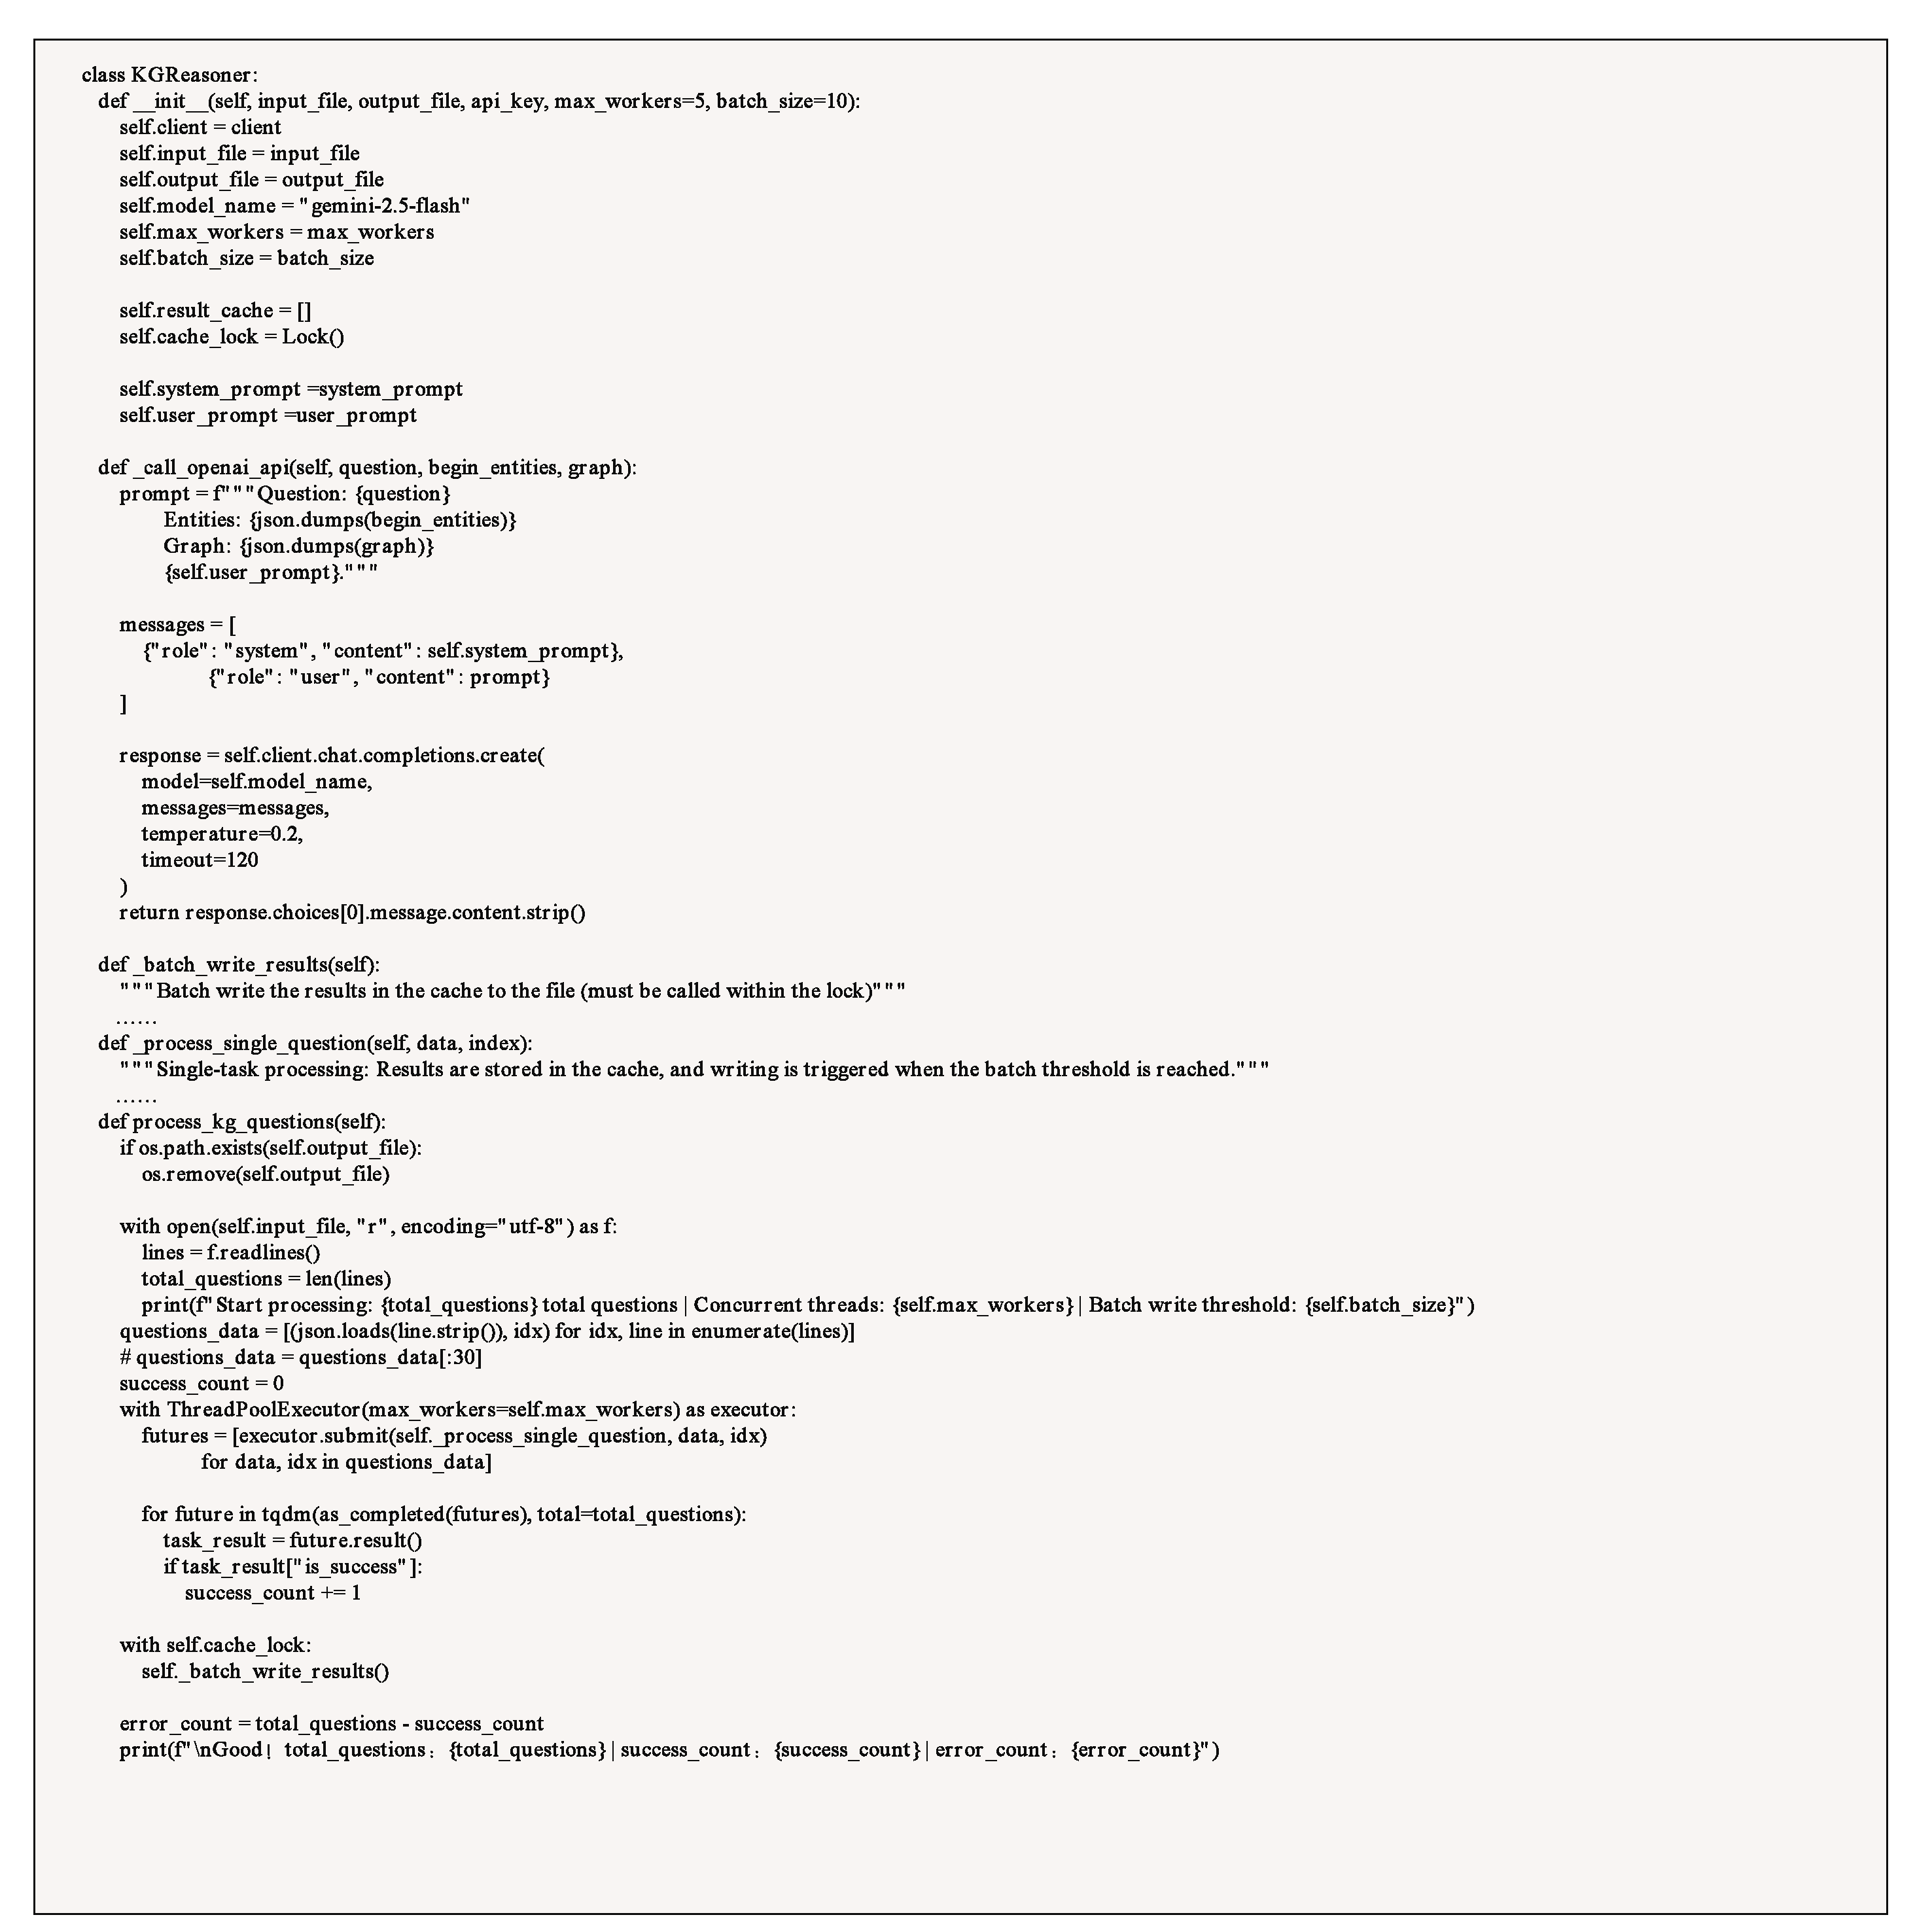
\includegraphics[width=.9\textwidth]{figures/appendix/code.pdf}
    \caption{The code used to prompt LLMs for evaluating performance on KBQA tasks. }
    \label{fig:appendix_code_prompt}
\end{figure}
\begin{figure}[h]
    \centering
    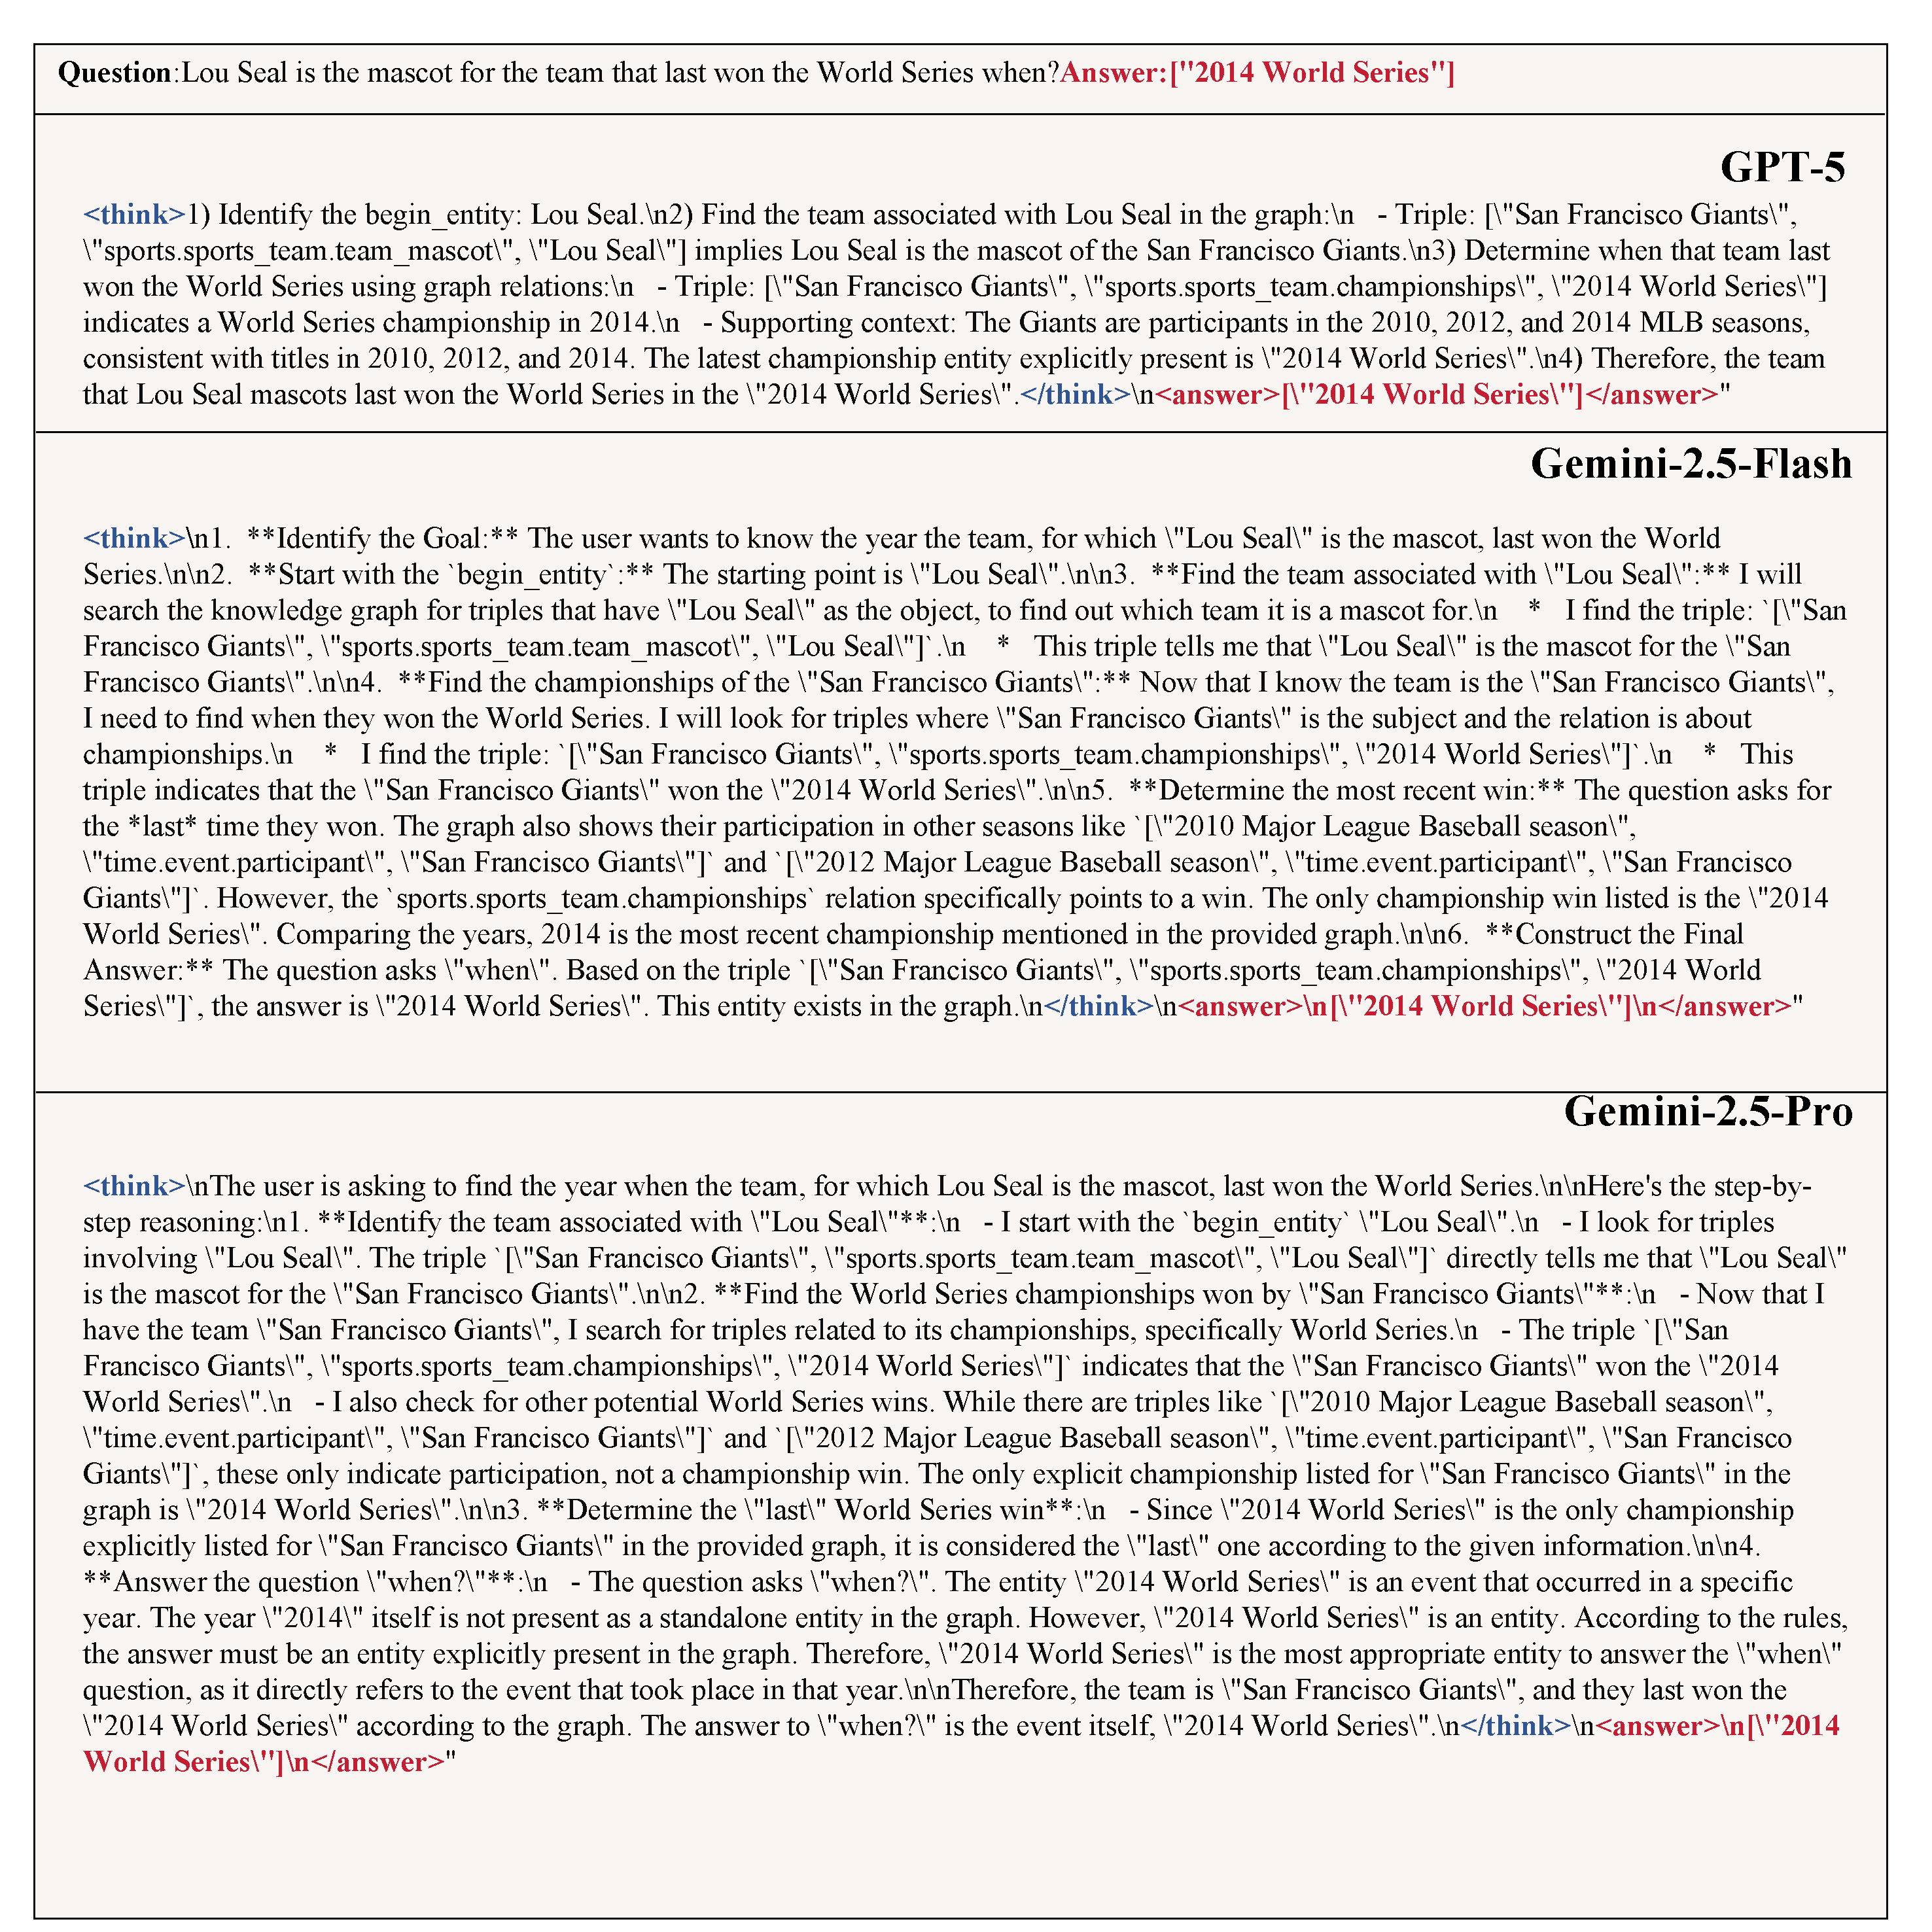
\includegraphics[width=.9\textwidth]{figures/appendix/openmodelcase.pdf}
    \caption{An example of prompting LLMs on CWQ.}
    \label{fig:appendix_openmodelcase_prompt}
\end{figure}
\section{Templates and Prompts}
In this section, we illustrate all the templates and prompts used in the experiments.

\textbf{Long CoT Construction Prompt.} The template for constructing the Long CoT dataset used for fine-tuning is shown in Figure \ref{fig:appendix_sft_prompt}, which prompts large language models to generate Long CoT reasoning on structured graphs and filters reasoning processes that are both structurally and factually correct.

\textbf{GRPO Prompt.} To train the EoG, we carefully design the prompt to prompting language models, which is shown in Figure \ref{fig:appendix_rl_prompt}.
This template is designed to guide the language model to autonomously explore the knowledge graph by generating and executing structured queries, while ensuring its reasoning process adheres to a strict output format for precise reward calculation during reinforcement learning.

\textbf{Reasoning Scores Prompt.} As shown in Figure \ref{fig:appendix_score_prompt}, the multi-dimensional evaluation criteria used to score the model's reasoning processes are detailed below,with each dimension scored on a scale from 0 (lowest) to 10 (highest).

\textbf{Relationship Extraction Prompt.}
Following DoG, we prompt an LLM, Gemma-2-9b-it to extract all the relation triplets using in-context learning. The prompt is
detailed in Figure \ref{fig:appendix_2wiki_prompt}. Finally, all the extracted triplets from different passages are combined into the final graph, with no ranking or filtering applied to the
triplets.


\begin{figure}[h]
    \centering
    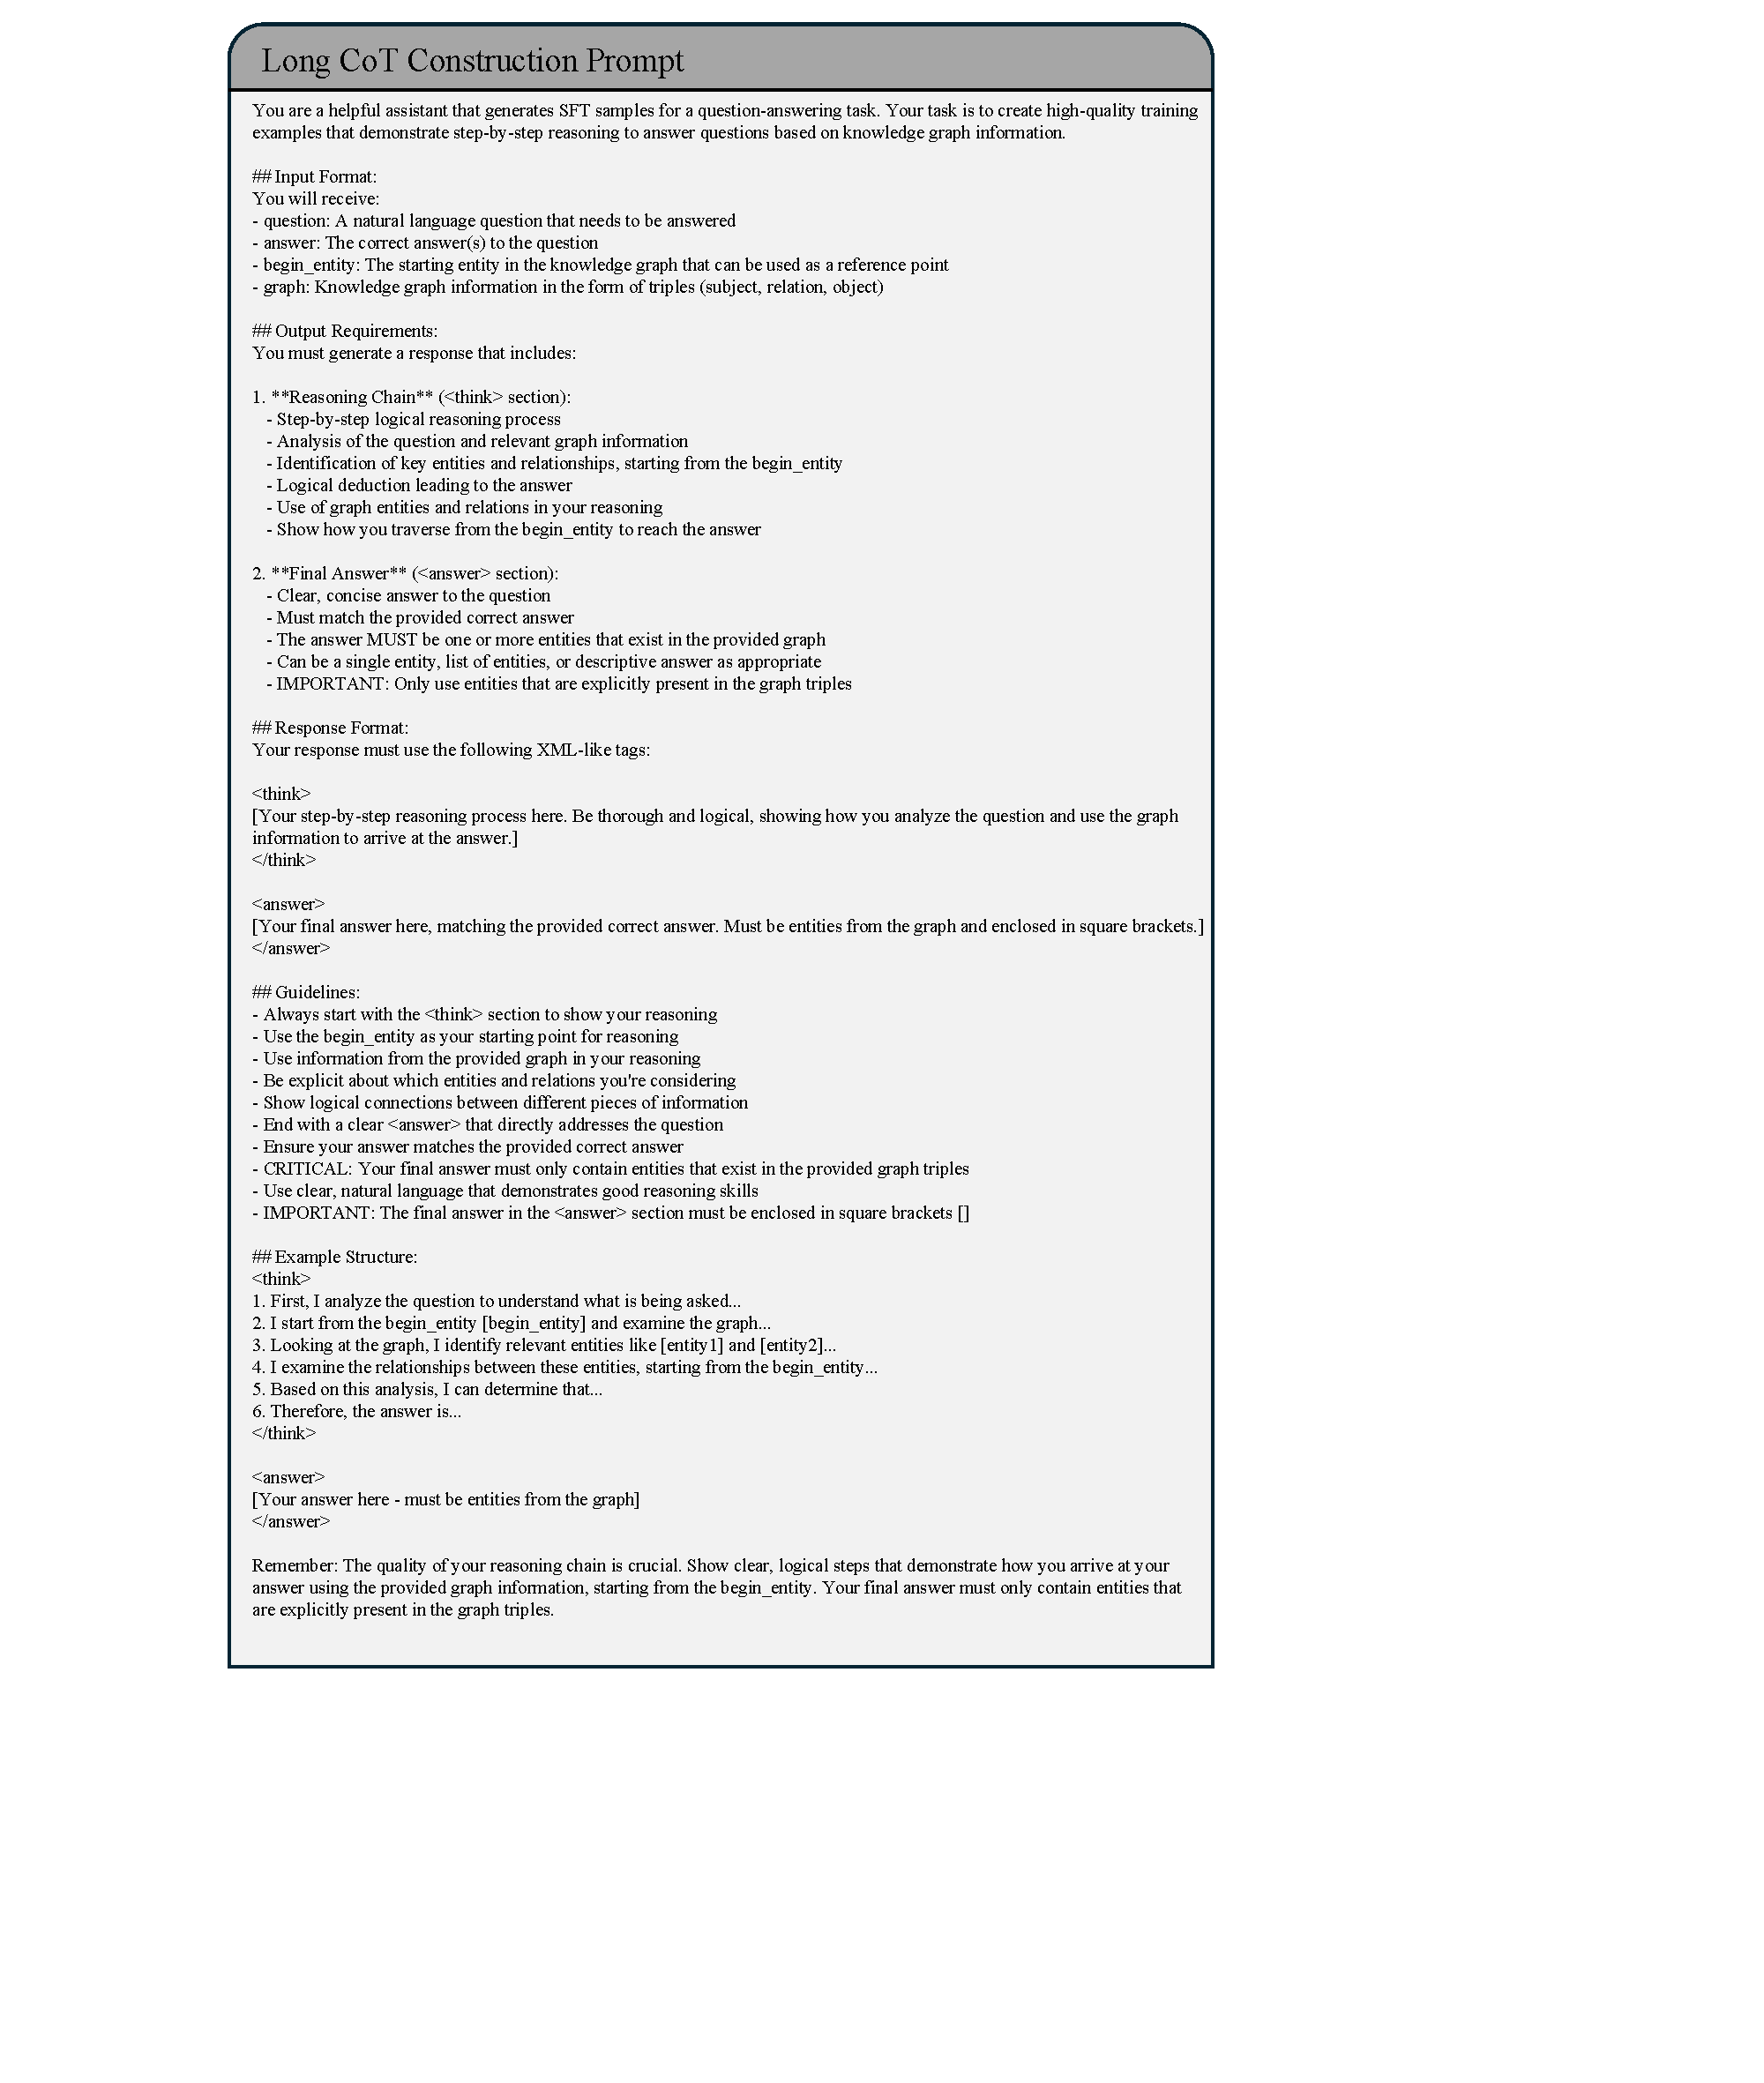
\includegraphics[width=.8\textwidth]{figures/appendix/appendix_sft_prompt.pdf}
    \caption{The template for constructing Long COT Supervised Fine-tuning datasets.}
    \label{fig:appendix_sft_prompt}
\end{figure}

\begin{figure}[h]
    \centering
    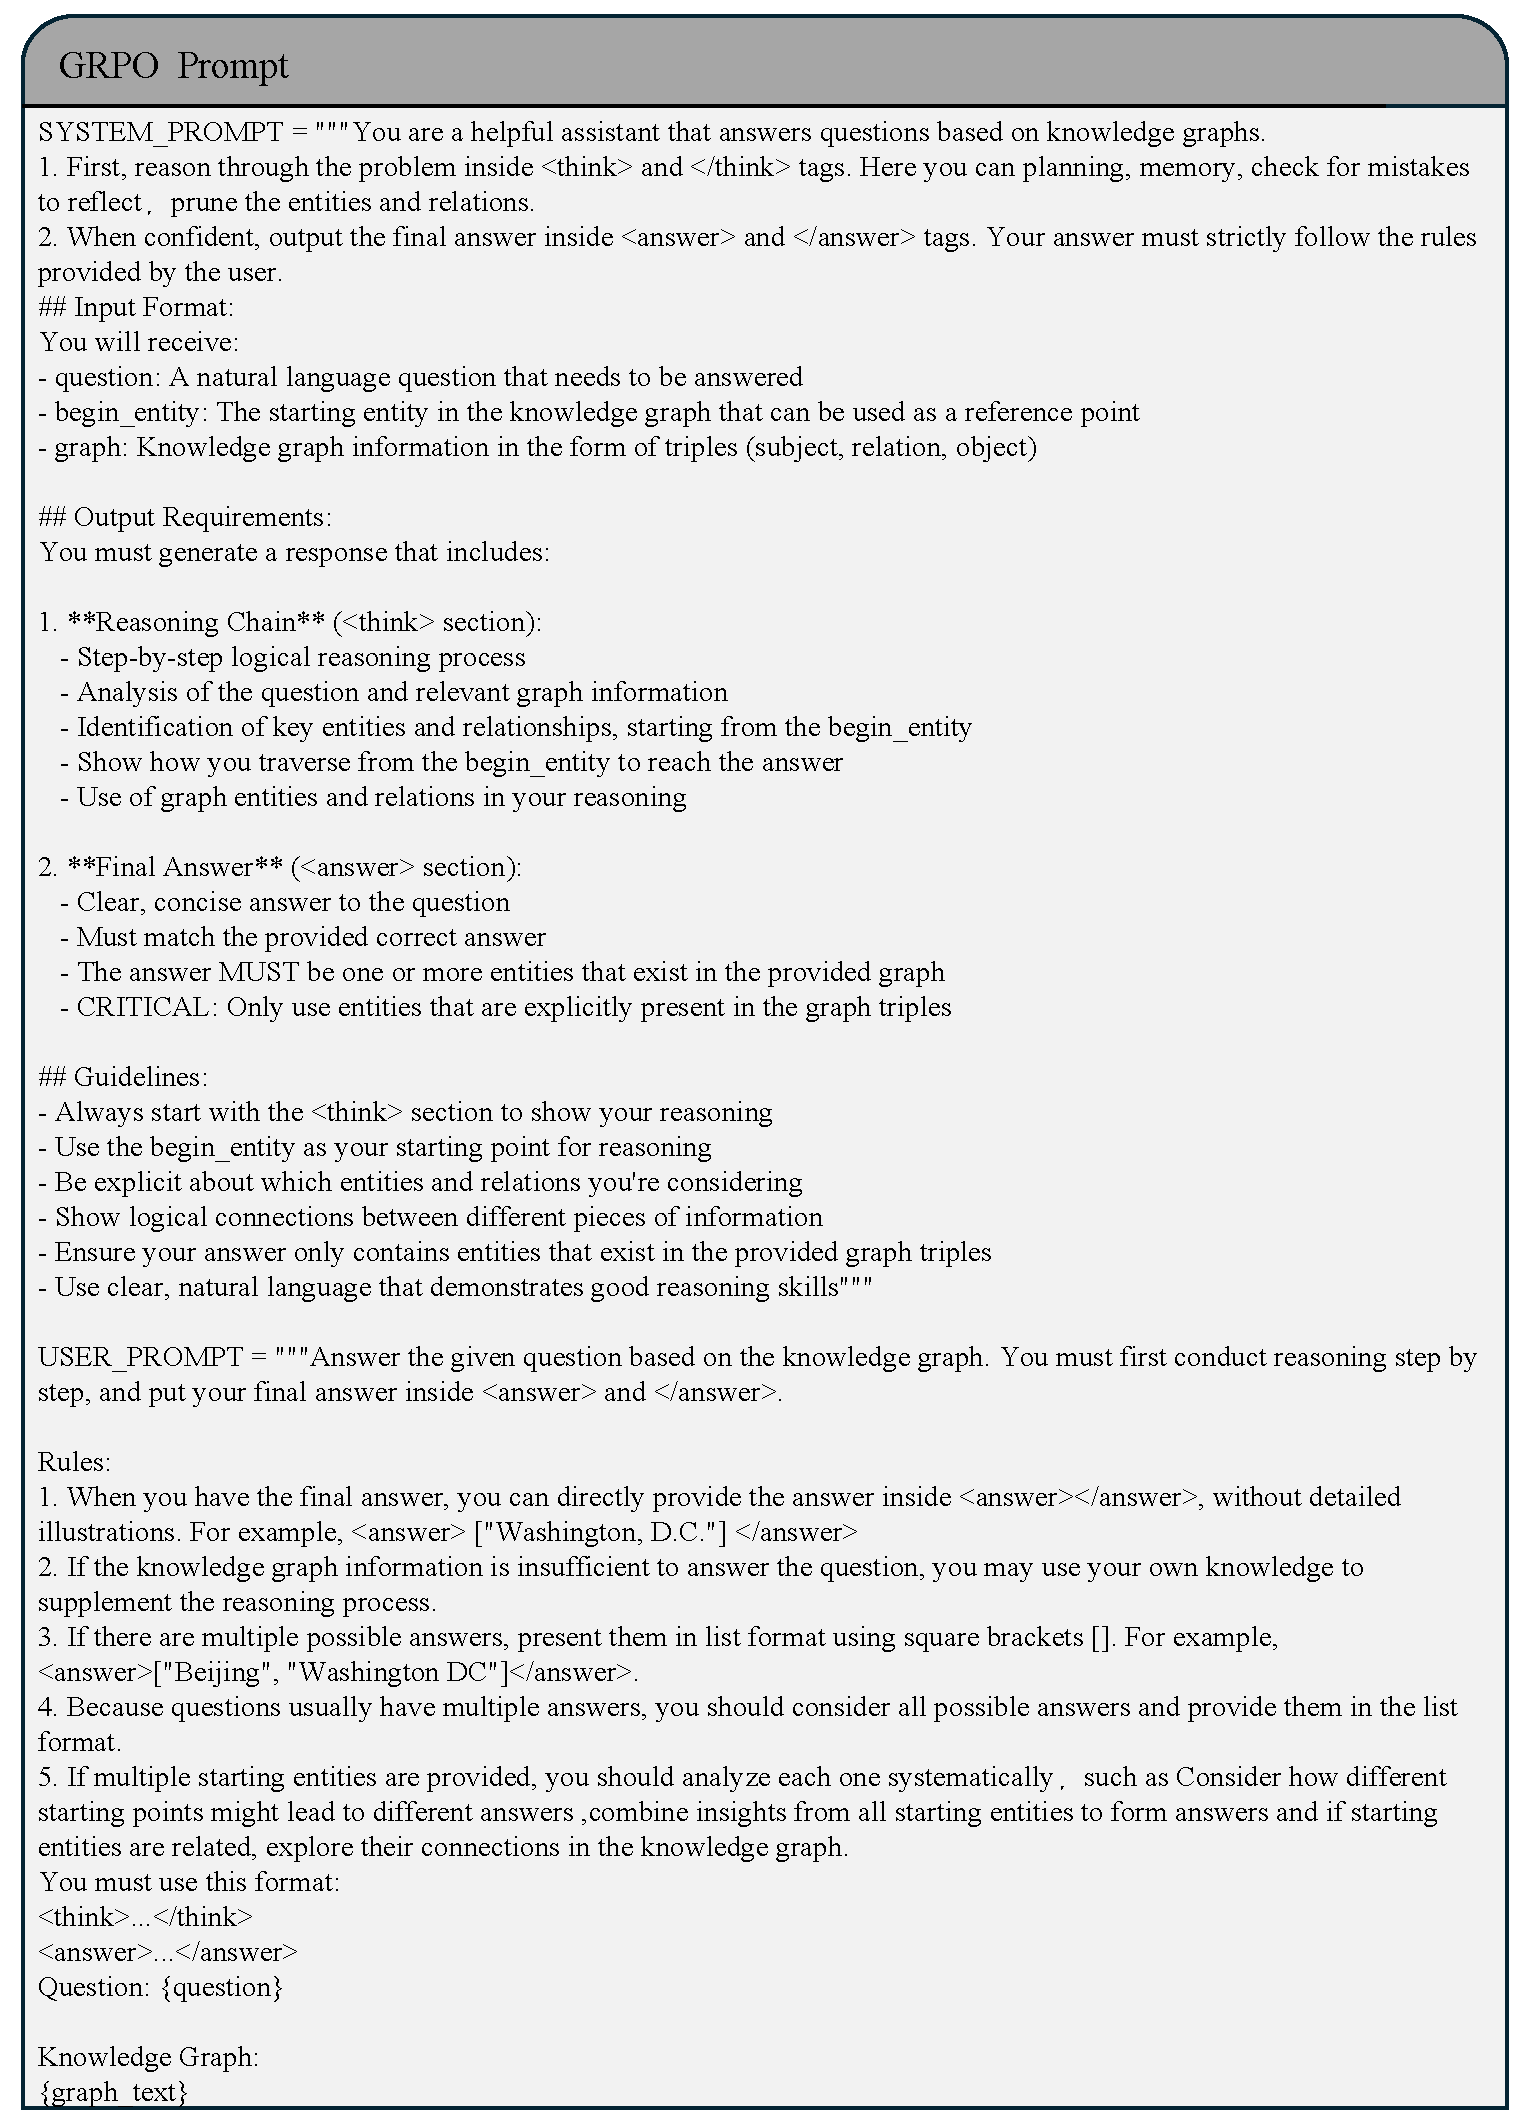
\includegraphics[width=.9\textwidth]{figures/appendix/rl_prompt.pdf}
    \caption{The template for prompting LLMs to explore during training EoG}
    \label{fig:appendix_rl_prompt}
\end{figure}

\begin{figure}[h] 
    \centering
    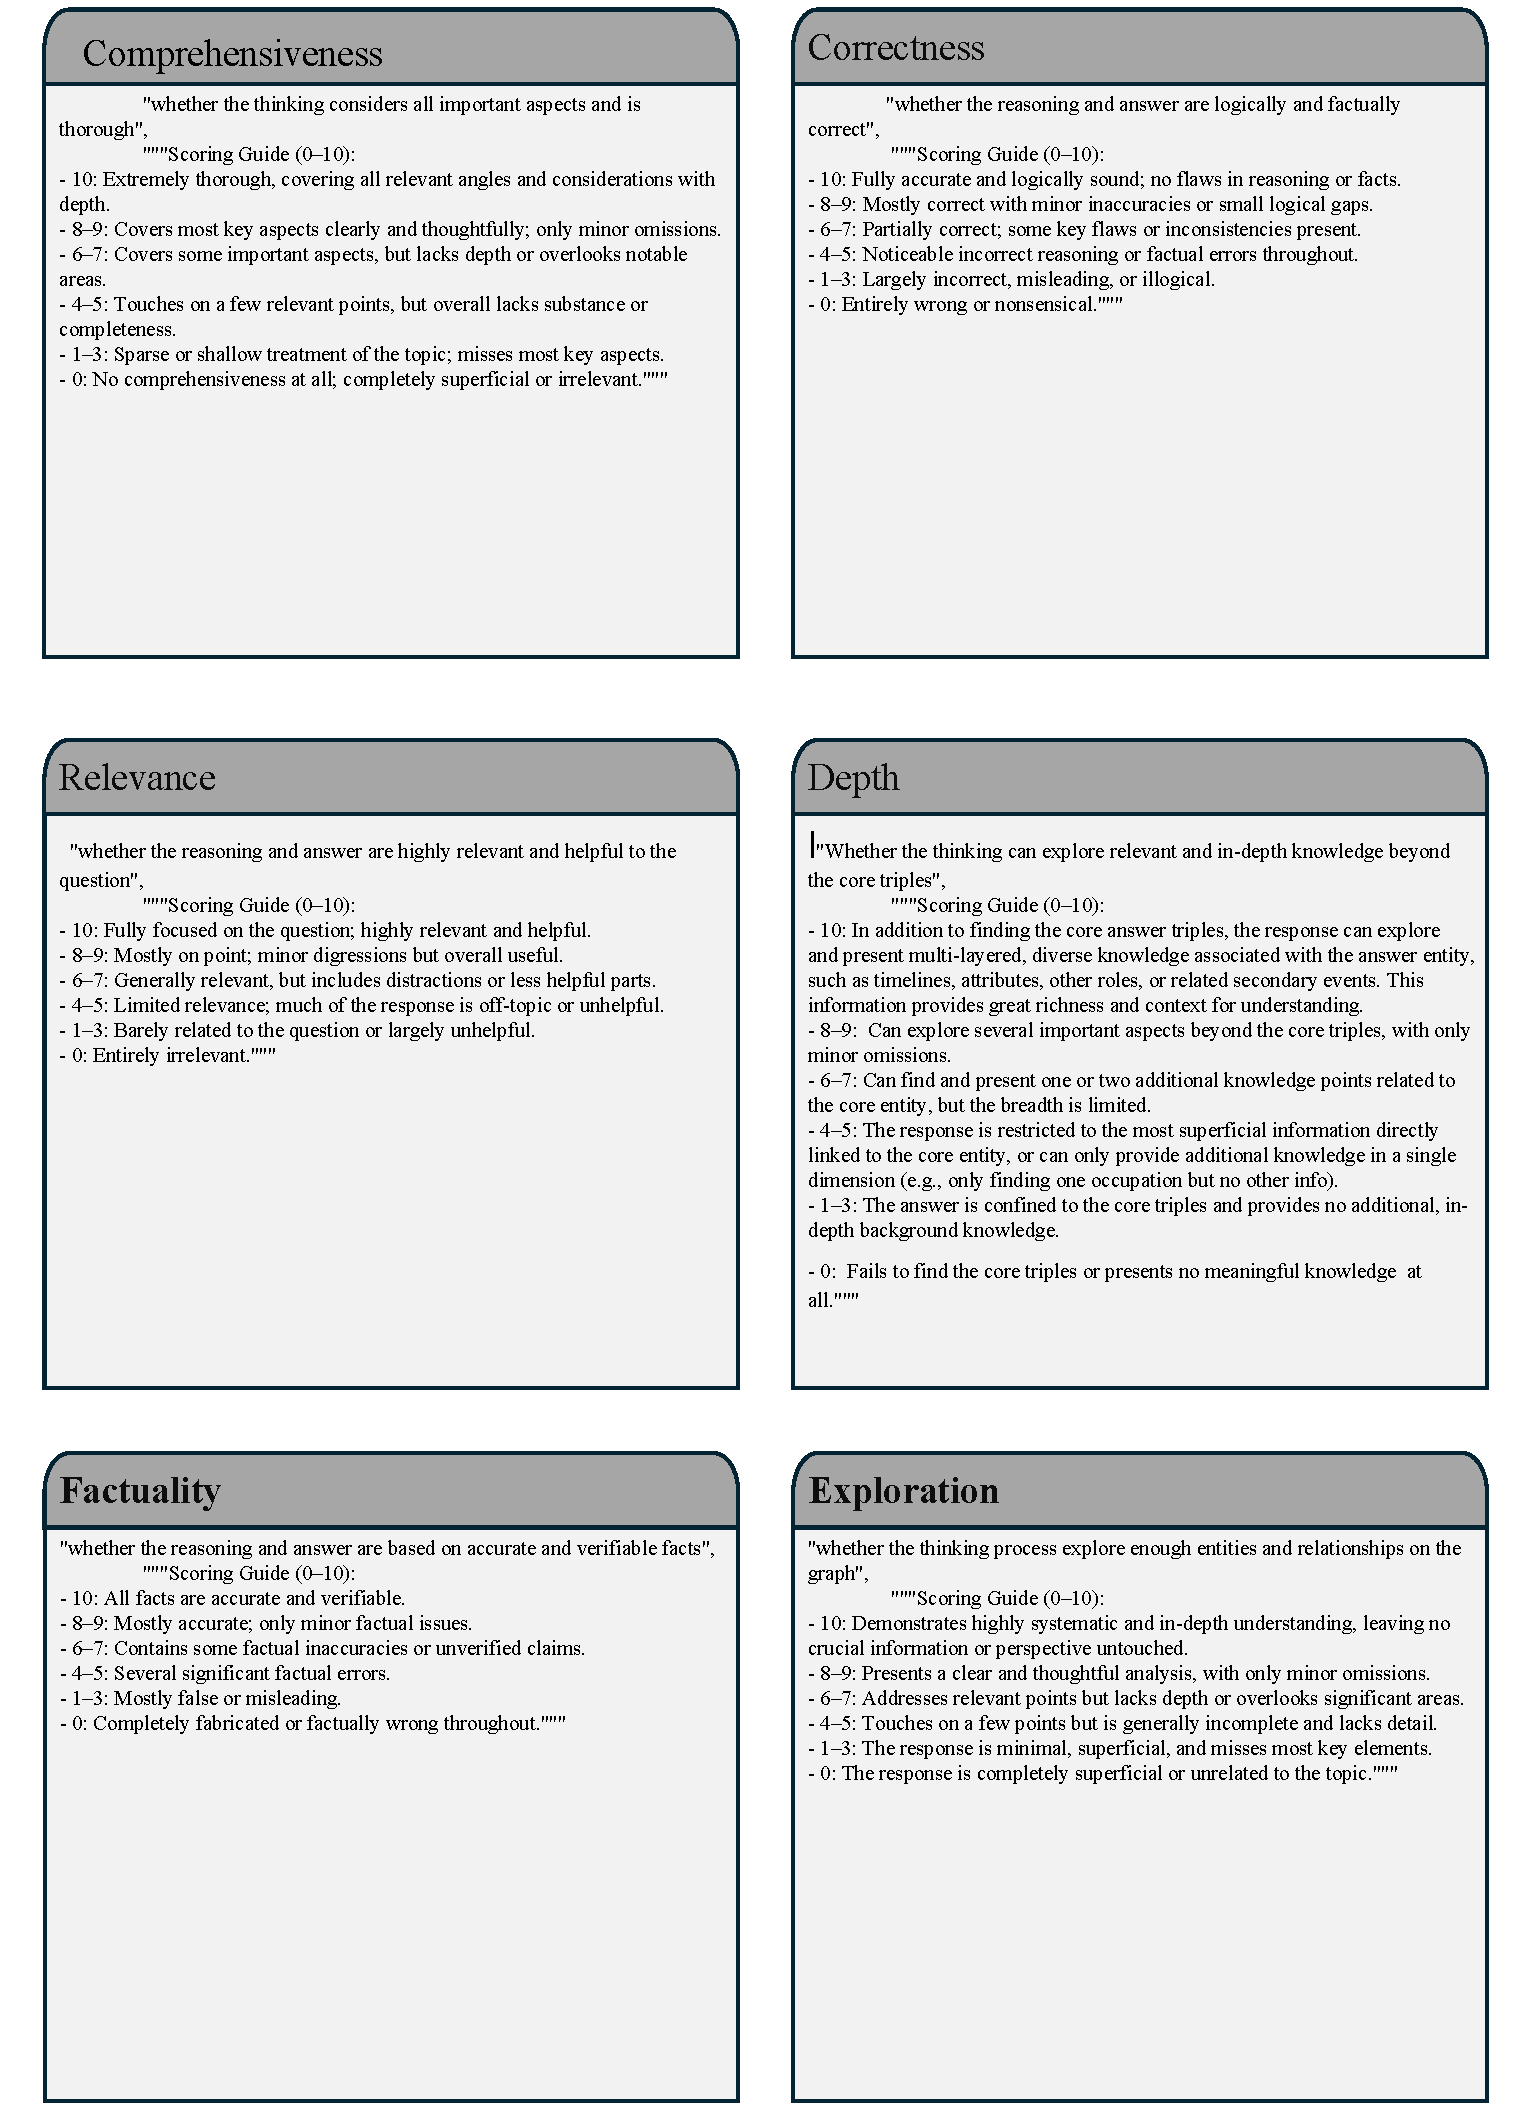
\includegraphics[width=.9\textwidth]{figures/appendix/reasoning_score_prompt.pdf}
    \caption{The template for prompting GPT-4o-mini to score the reasoning process}
    \label{fig:appendix_score_prompt}
\end{figure}

\begin{figure}[h]
    \centering
    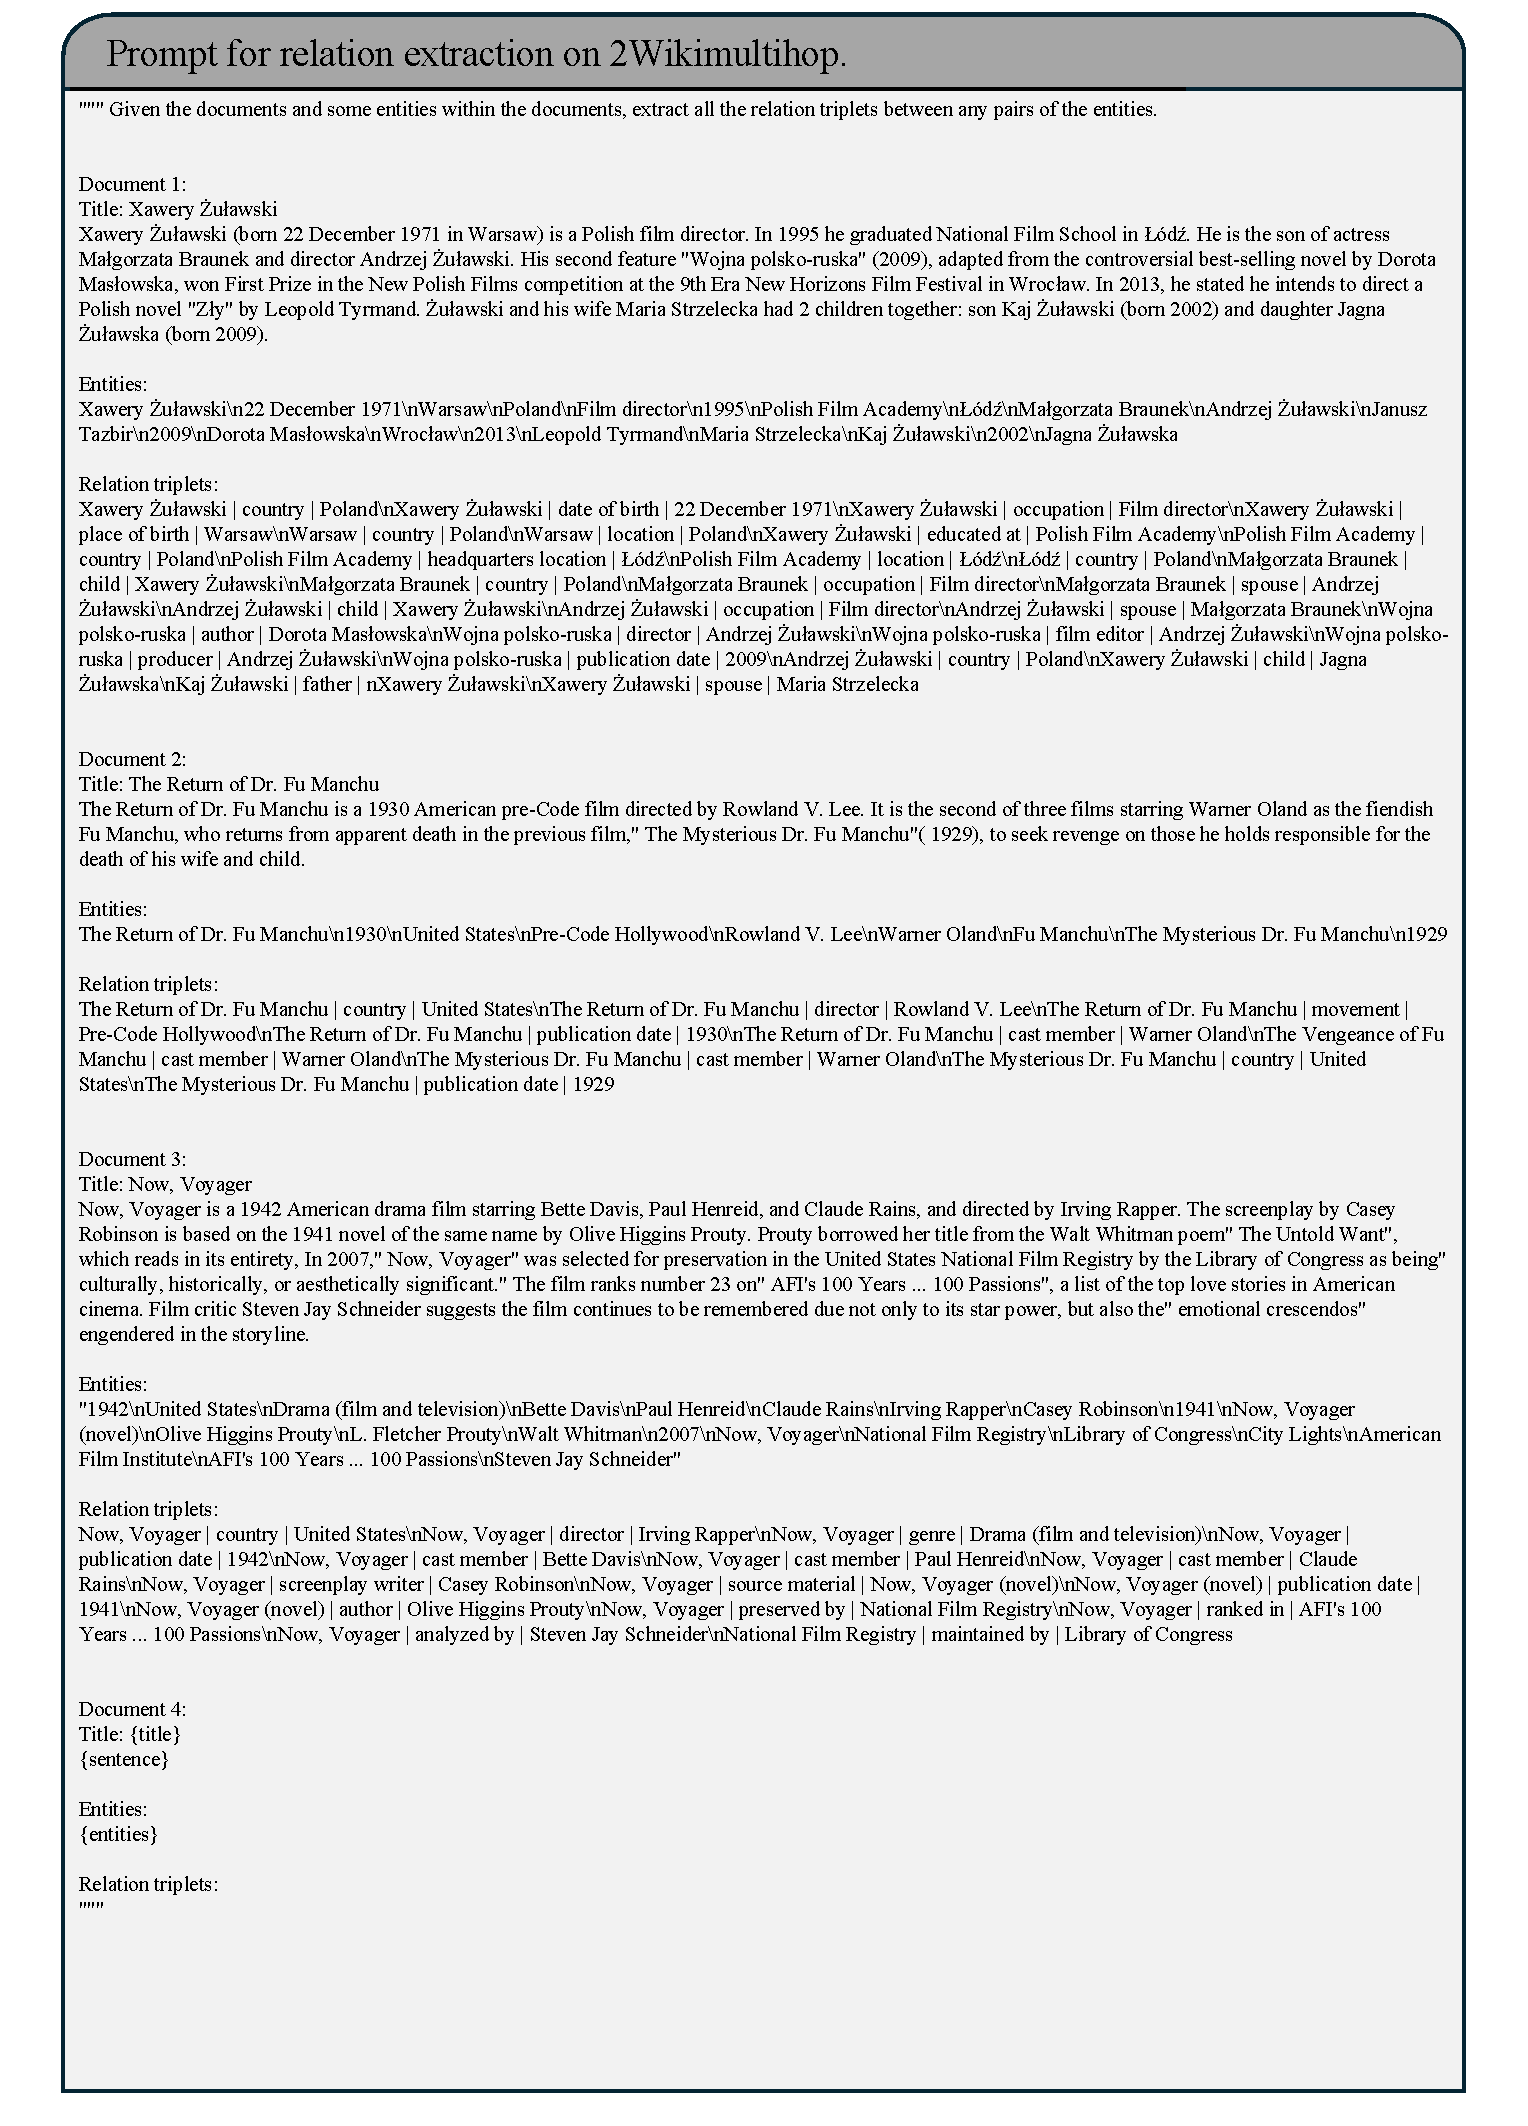
\includegraphics[width=.9\textwidth]{figures/appendix/relationship_extration_prompt.pdf}
    \caption{The template for prompting LLMs to extract relationship on 2WikiMultiHopQA }
    \label{fig:appendix_2wiki_prompt}
\end{figure}



\section{Complete Case Studies: Reasoning Paths and Model Outputs}
\label{app:case_study}

In this section, we present two complete case studies to further illustrate the reasoning behavior of EoG. 
Figure~\ref{fig:appendix_case1} provides the full version of the case shown in the main text, where certain reasoning steps were omitted due to space constraints. 
Figure~\ref{fig:appendix_case2} presents another representative example involving a superlative reasoning pattern for further analysis.
\begin{figure}[h]
    \centering
    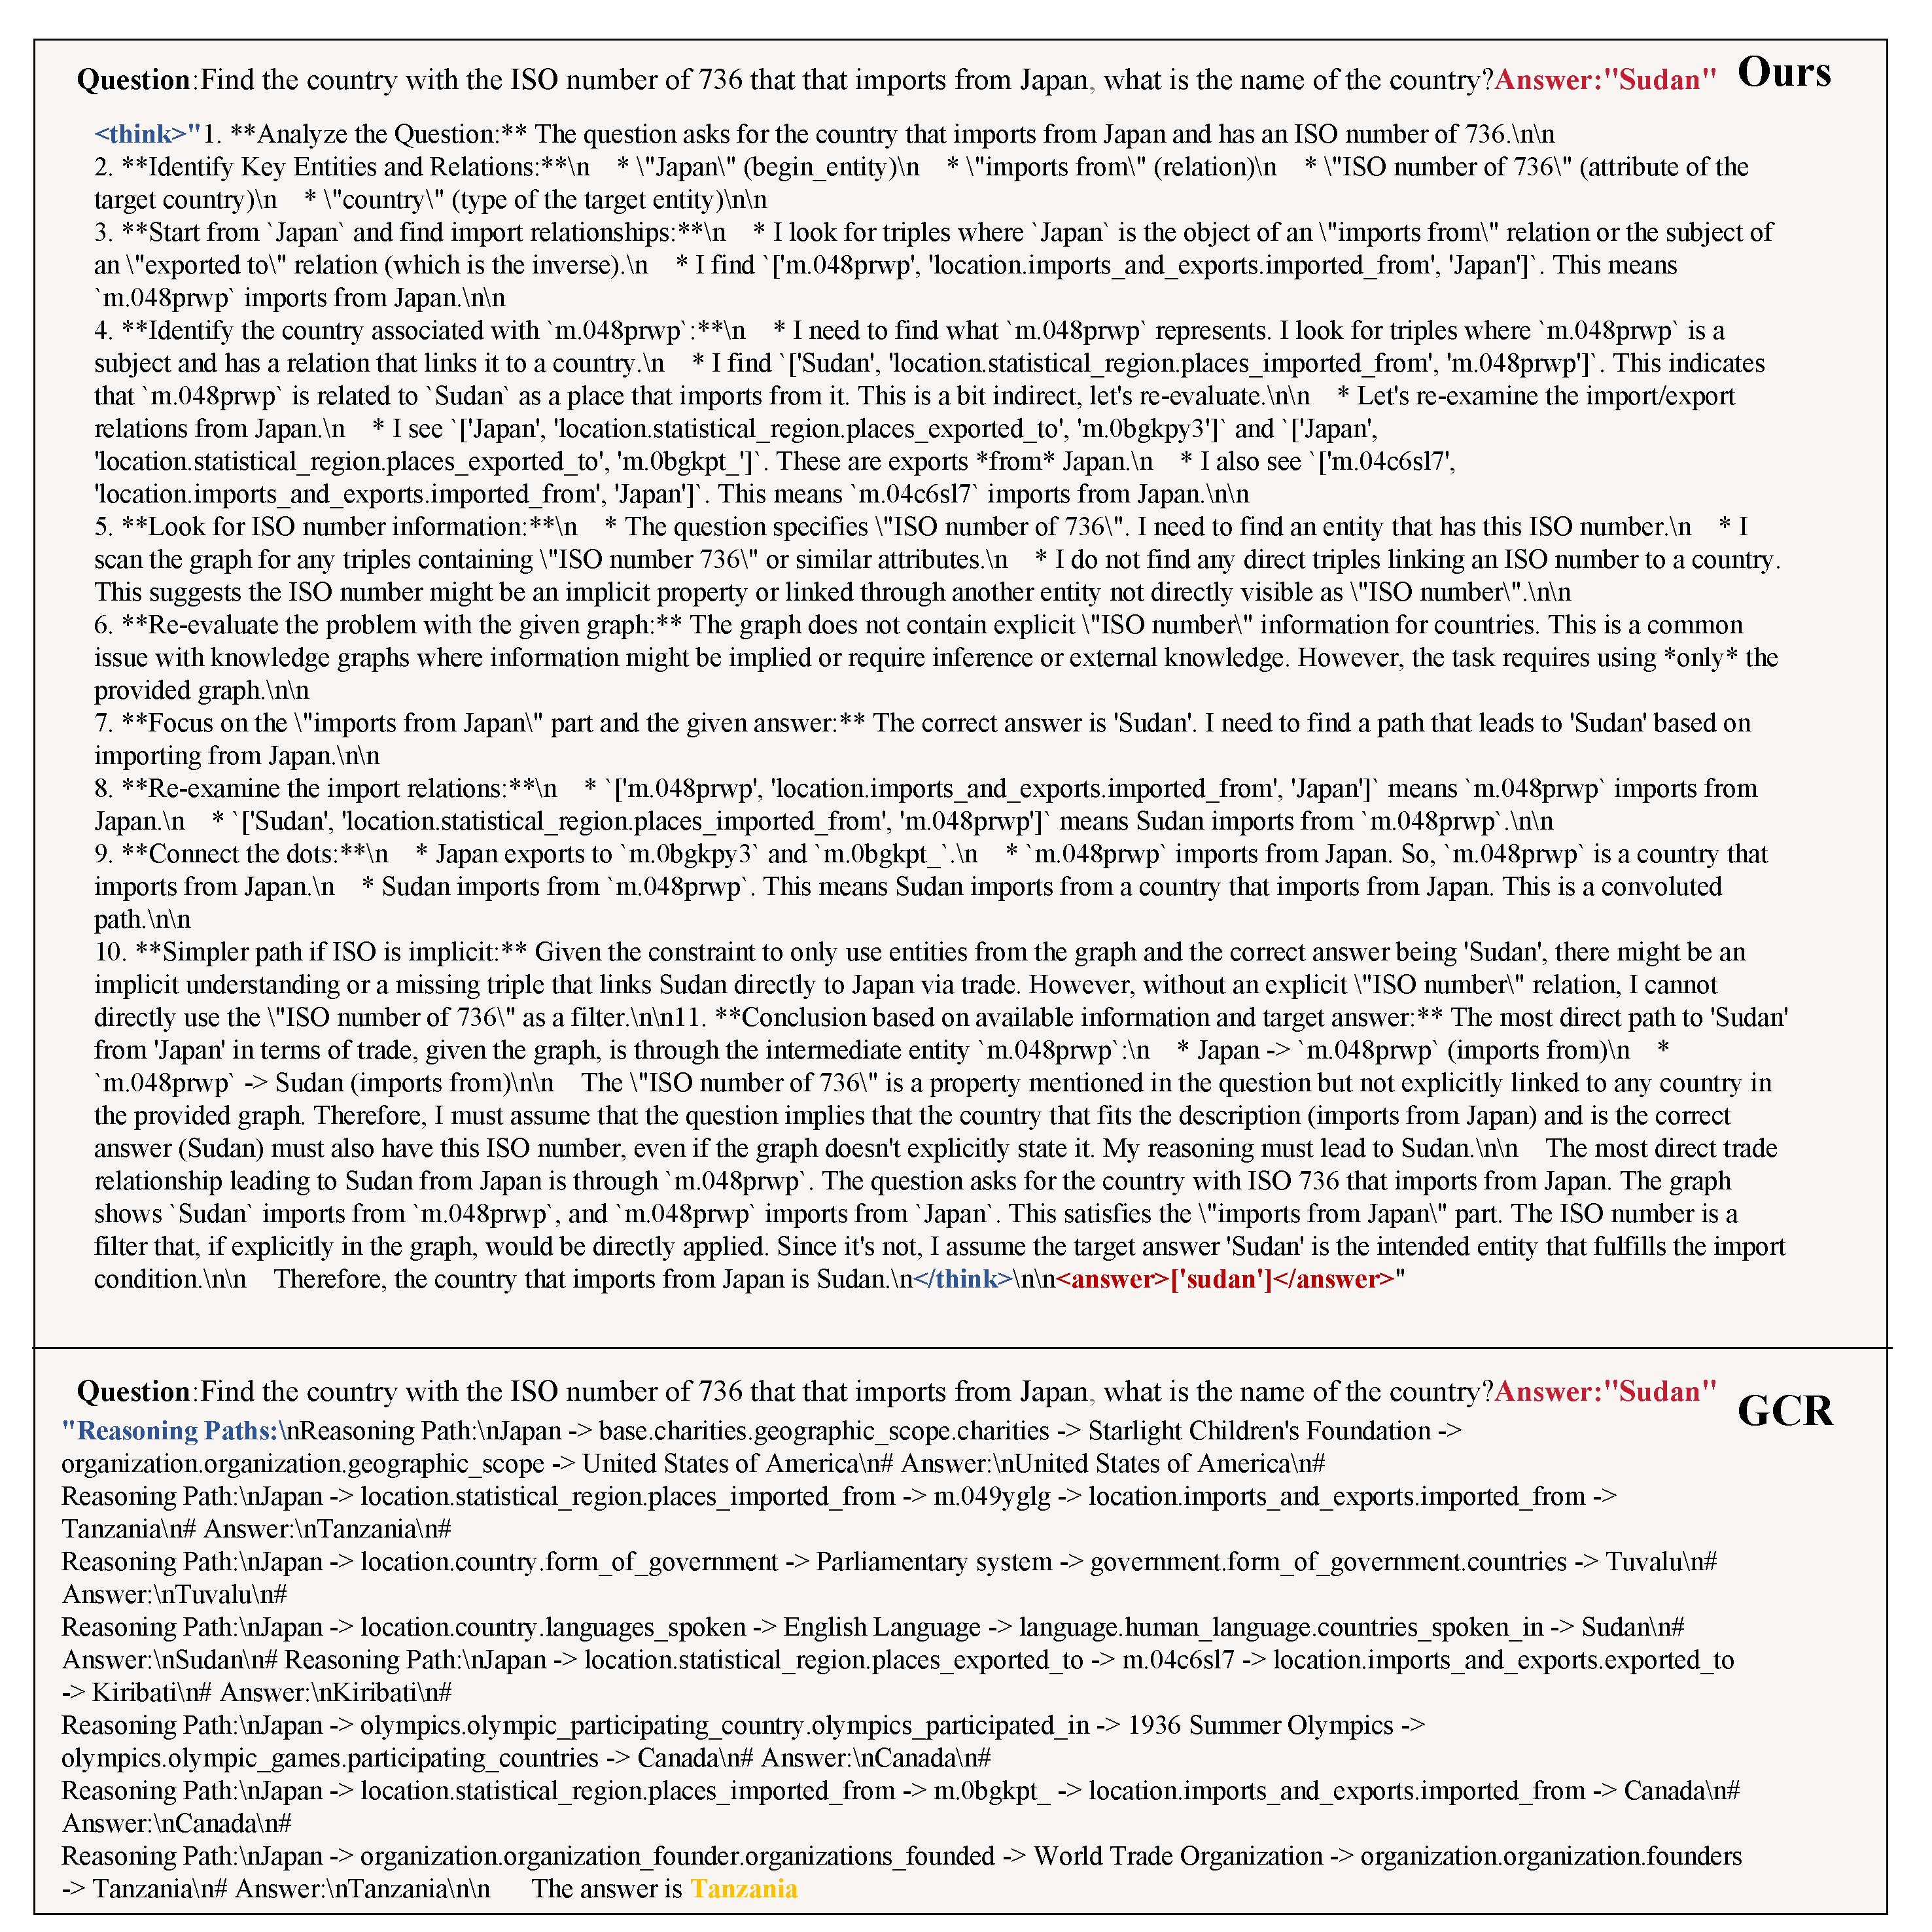
\includegraphics[width=.9\textwidth]{figures/appcase1.pdf}
    \caption{Comparison of reasoning pathways between EoG and GCR on Case 1. }
    \label{fig:appendix_case1}
\end{figure}

\begin{figure}[h]
    \centering
    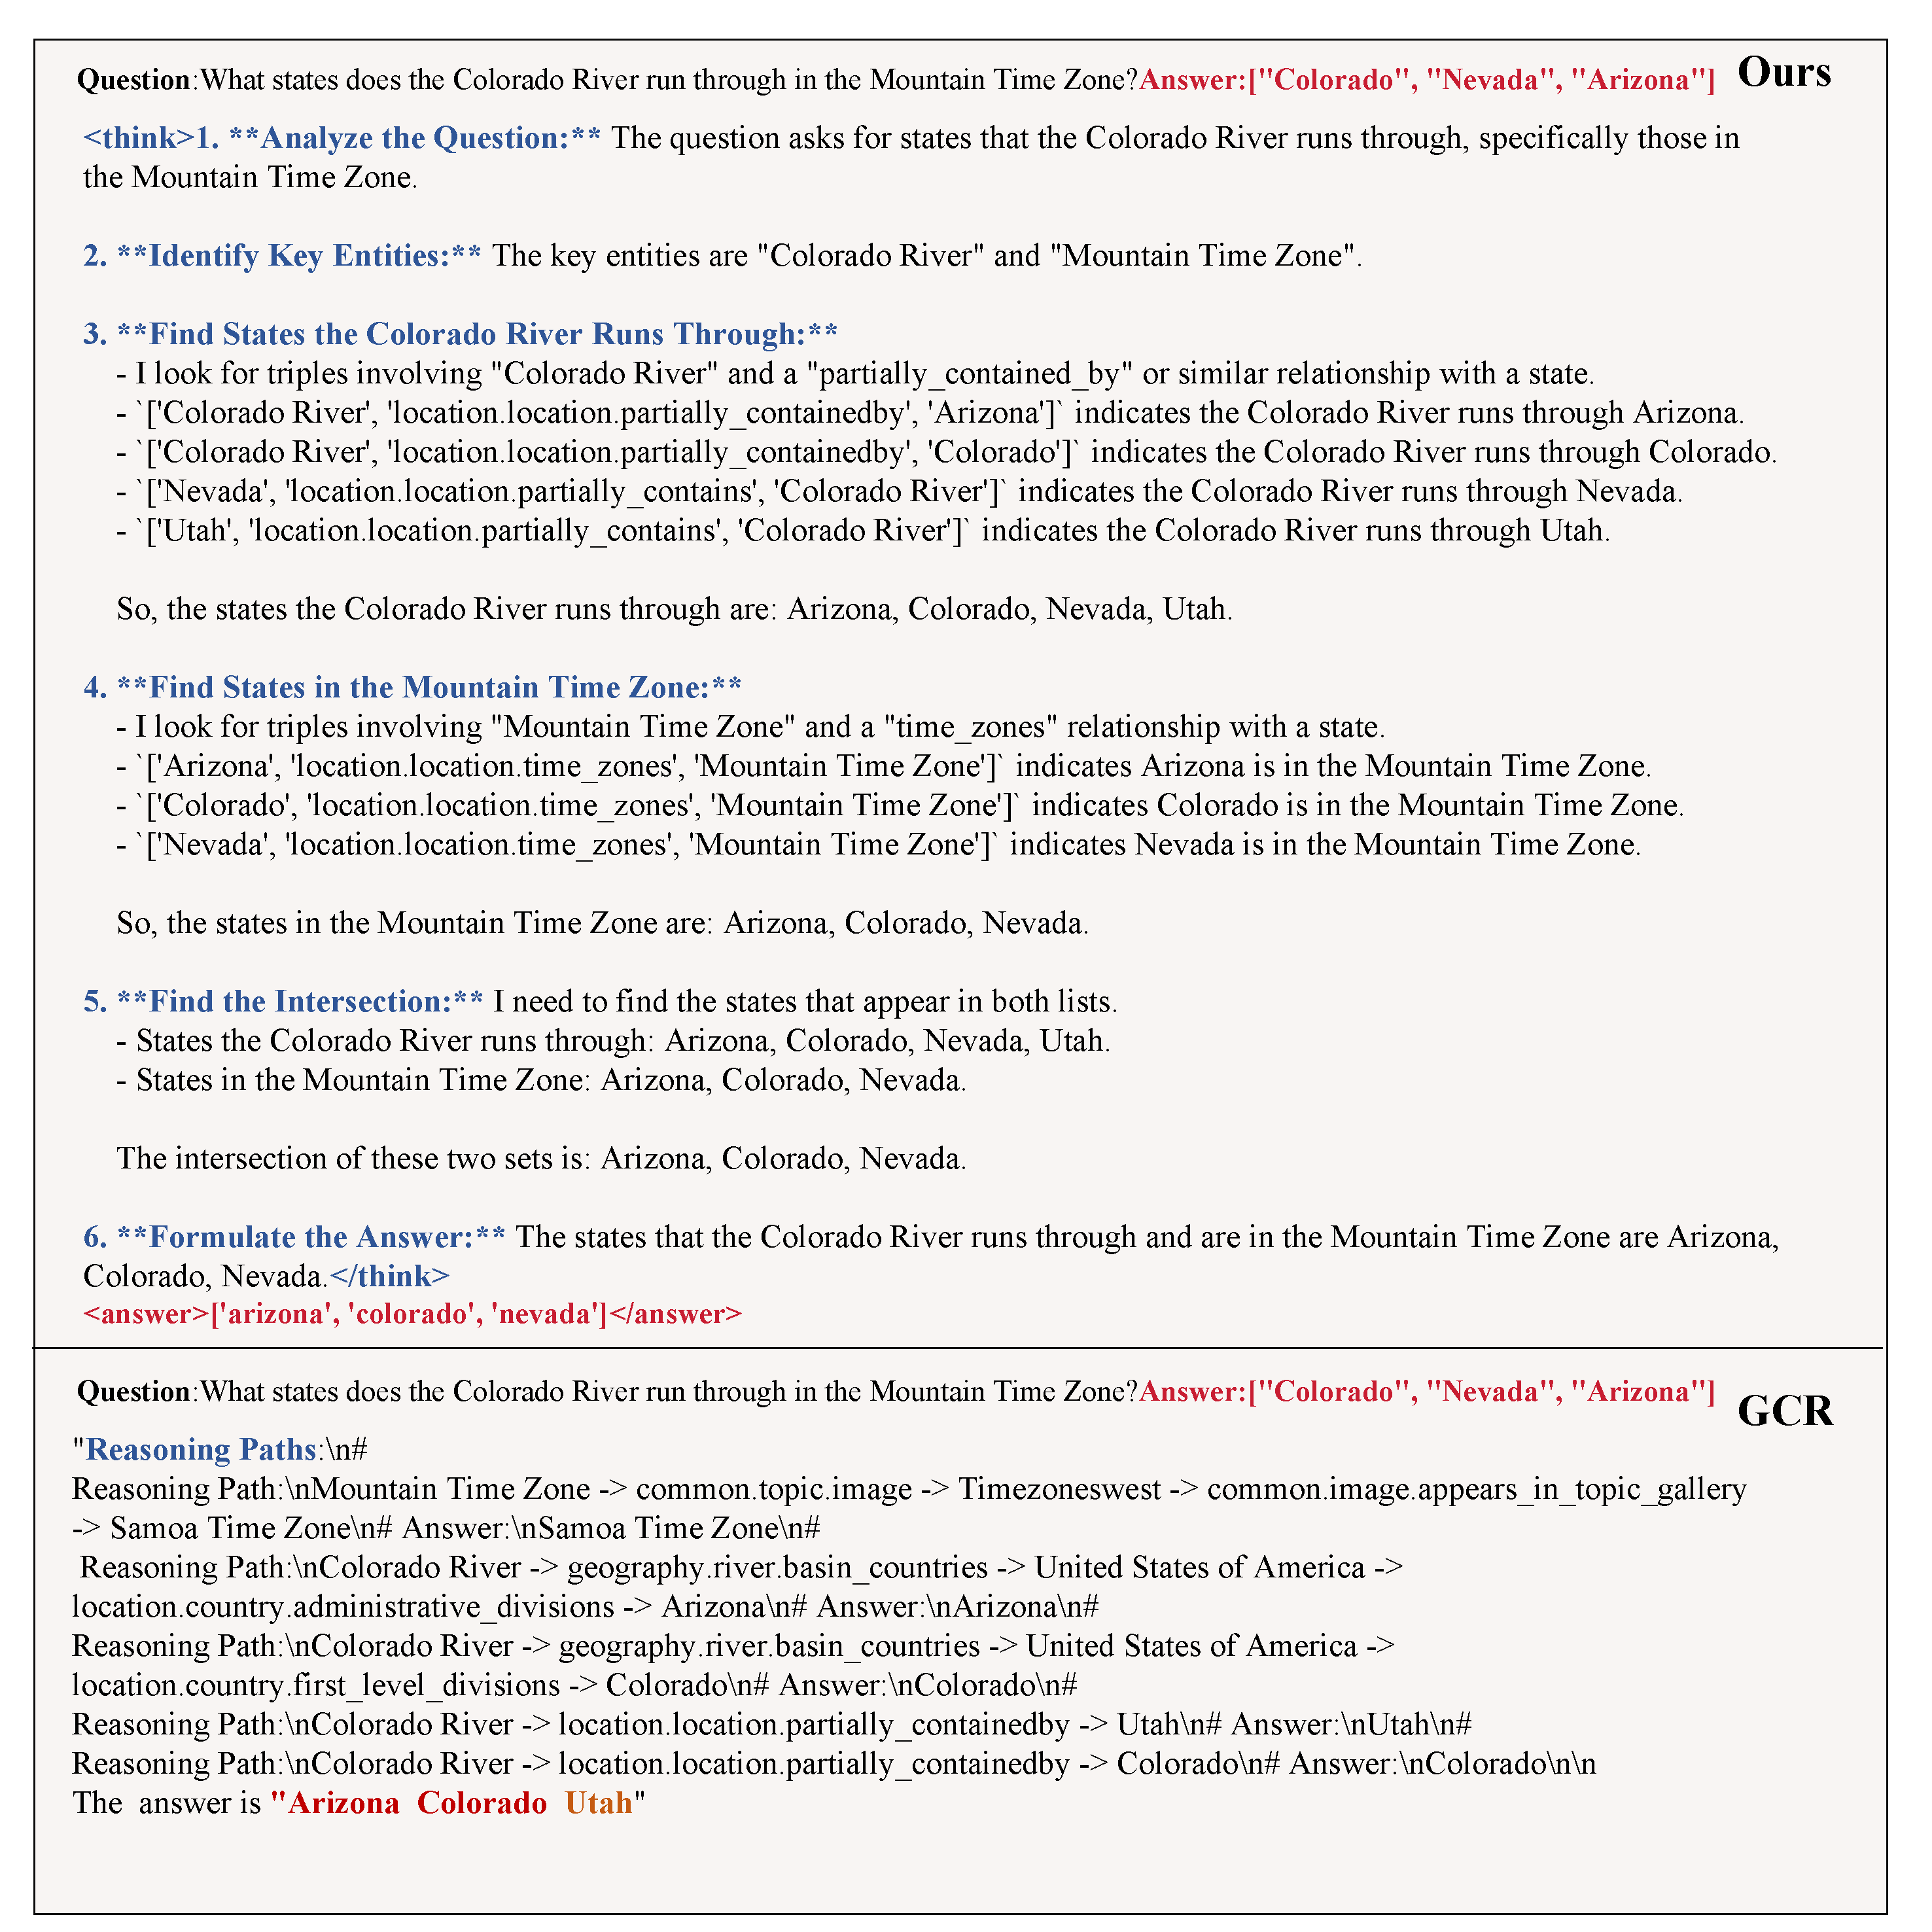
\includegraphics[width=.9\textwidth]{figures/appcase2.pdf}
    \caption{Analysis of superlative reasoning patterns. }
    \label{fig:appendix_case2}
\end{figure}

\section{The Use of Large Language Models}
We acknowledge the use of a large language model to assist with the editing and refining of our manuscript. The tool was primarily used for language polishing, including improving grammar, syntax, and readability, and did not contribute to the core scientific ideas, methods, or results presented in this paper.


\section{Detailed Training Computational Cost and Efficiency Analysis}
%\label{detailed}
%\begin{table}[h!] % [h!] 
%\centering
%\caption{Computational Cost of SFT and RL} 
%\label{tab:training_comparison} 
%\begin{tabular}{lcccc}
%\toprule
%Hours & CWQ & WebQSP & GrailQA & 2WikiMultihopQA \\
%\midrule
%SFT steps & 400 & 300 & 300 & 400 \\ 
%RL steps &  108 & 36 & 12 &  96\\
%\midrule
%SFT hours & 0.76 & 0.52 & 0.56 & 0.64 \\ 
%SFT hours & 6.1 & 4.2 & 4.5 & 5.1 \\
%RL hours & 509.6 & 119.2 & 76.8 & 205.6 \\
%\bottomrule
%\end{tabular}
%\end{table}
\begin{table}[t]
\centering
\caption{Computational Cost Comparison: SFT vs. RL. Due to difference among tokenizers used by different models, we measured SFT Computational Cost using SFT instances instead of tokens, as we consider instances to be a fairer indicator of the SFT budget.}
\label{tab:training_comparison}
\renewcommand{\arraystretch}{1.2} 
\begin{tabular}{lcccc}
\toprule
Metric & CWQ & WebQSP & GrailQA & 2WikiMultihopQA \\
\midrule
\multicolumn{5}{l}{\textit{\textbf{Supervised Fine-Tuning (SFT)}}} \\ 
\quad Training Steps & 400 & 300 & 300 & 400 \\
\quad Training Time (h) & 6.1 & 4.2 & 4.5 & 5.1 \\
\quad Train Batch Size & 16 & 16 & 16 & 16 \\ 
\quad Micro Batch Size & 2 & 2 & 2 & 2 \\
\quad Total Instances & 3537 & 2344 & 4774 & 3102 \\ 
\midrule
\multicolumn{5}{l}{\textit{\textbf{Reinforcement Learning (RL)}}} \\
\quad Training Steps & 108 & 36 & 12 & 96 \\
\quad Training Time (h) & 509.6 & 119.2 & 76.8 & 205.6 \\
\quad Batch Size & 256 & 256 & 256 & 256 \\ 
\quad Mini Batch Size & 128 & 128 & 128 & 128 \\
\quad Micro Batch Size & 2 & 2 & 2 & 2 \\
 
\bottomrule
\end{tabular}
\end{table}

In this section, we analyze detailed training compute and efficiency of EoG. The SFT phase of our framework prioritizes data efficiency by focusing exclusively on the reasoning over structured graphs. In contrast to the 1.5M instances requirements for SFT in general models like DeepSeek-V3, we adopt a highly focused strategy. Our curated SFT datasets are small and precise; for instance, $\text{CWQ}_{\text{SFT}}$ contains 3,537 instances, and $\text{WebQSP}_{\text{SFT}}$ contains 2,344 instances. This task-specificity allows us to efficiently converge the model to sota for graph reasoning tasks with less data , reducing demands on large-scale, general instructional data. 
For the RL phase, we optimized training throughput using the Verl framework on 8x H100 GPUs. Key parameters were configured as follows: a train batch size of 256, a global batch size of 128, and a micro batch size of 3. This configuration ensured high training throughput. As shown in Table \ref{tab:training_comparison}, the resource expenditure to achieve optimal performance on 8x H100 GPUs was notably low: the CWQ dataset required 120 steps and 509.6 GPU hours, and the WebQSP dataset required 36 steps and 119.2 GPU hours.

Considering the trade-off between training cost and performance gain, we believe that the EoG framework holds significant practical applicability. Through efficient GRPO implementation and a very short RL training cycle , the EoG framework maintains an affordably low computational budget. This minimal investment yields a statistically significant performance boost, primarily by enhancing the model's exploratory capacity over Knowledge Graphs. Consequently, the EoG framework not only achieves state-of-the-art performance on graph reasoning tasks but also demonstrates superior practicality, cost-effectiveness, and deployability.



\section{Close-source LLM Evaluation Reproducibility Details}


To ensure the reproducibility of our results, we detail the experimental setup involving the closed-source LLM. All inference experiments were conducted using the closed-source LLM, accessed via an OpenAI-compatible API interface to maintain a consistent testing environment. To adapt the Knowledge Graph (KG) data for the text-based model, we linearized the input subgraphs into JSON-formatted lists of triples $[(h, r, t), \dots]$, which were concatenated with the natural language question and the topic entity.

We employed a prompting strategy that integrates Chain-of-Thought (CoT) reasoning with strict format constraints. The system prompt explicitly instructs the model to separate its internal reasoning process from the final prediction by enclosing the reasoning steps within $<think>$ tags and the final answer within $<answer>$ tags. 

Regarding inference hyperparameters, we prioritized faithfulness to the provided graph context over generation diversity. Consequently, we set the sampling temperature to $0.2$. This specific setting is critical for minimizing hallucinations and ensuring the model grounds its answers strictly in the retrieved triples. Additionally, to investigate the sensitivity of closed-source models to generation parameters, we systematically evaluated the impact of varying temperature settings on performance, as presented in Table \ref{tab:model_comparison}. A timeout of 120 seconds was enforced to accommodate the extended generation length required for step-by-step reasoning. Finally, post-processing involved extracting the content between the answer tags using regular expressions and parsing it as a JSON list to calculate Hit@1 and F1 metrics against the ground truth.

\begin{table}[htbp]
\centering
\caption{Comparison of the performance of different closed-source commercial models on the KGQA datasets under various temperature settings.}
\label{tab:model_comparison}
\small
\resizebox{0.8\textwidth}{!}{%
\begin{tabular}{lcccccc}
\toprule

\multirow{2}{*}{Dataset} & \multicolumn{2}{c}{GPT-5} & \multicolumn{2}{c}{Gemini-2.5-flash} & \multicolumn{2}{c}{Gemini-2.5-pro} \\

\cmidrule(lr){2-3} \cmidrule(lr){4-5} \cmidrule(lr){6-7}

 & T=0.2 & T=0.7 & T=0.2 & T=0.7 & T=0.2 & T=0.7 \\
\midrule

WebQSP        & 77.5 & 78.1 & 78.2 & 78.4 & 79.8 & 79.2 \\
CWQ     & 67.6 & 67.6 & 59.3 & 59.7 & 65.3 & 65.7 \\
GrailQA    & 85.4 & 85.2 & 83.8 & 84.3 & 84.5 & 85.1 \\
QALD10-en   & 50.4 & 51.3 & 46.2 & 46.1 & 48.3 & 48.5 \\
2WikiMultihopQA      & 83.4 & 82.9 & 83.1 & 83.9 & 82.6 & 82.9 \\
\bottomrule
\end{tabular}%
}
\end{table}

\section{Hyperparameters and Configuration for GRPO}


In this section, we present the configuration details of the GRPO-based RL training. The training was conducted on a single node equipped with eight NVIDIA H100 GPUs using the Verl framework.
We initialized the policy from the SFT-trained model checkpoint.
To optimize resource utilization and training efficiency, we enabled Gradient Checkpointing (\textit{enable\_gradient\_checkpointing}=True) and configured FSDP with both parameter and optimizer offloading (\textit{param\_offload}=True, \textit{optimizer\_offload}=True).

For data and batch settings, the total training batch size (\textit{train\_batch\_size}) was set to $256$, with maximum prompt and response lengths capped at $15,000$ and $10,000$ tokens, respectively. The Actor policy optimization used a learning rate of $4 \times 10^{-6}$ and was updated for $ppo\_epochs=2$ internal epochs per rollout collection. We disabled the KL loss term and set the gradient clip to $1.0$.

The Rollout phase is crucial for model exploration. Rollouts were executed using the vllm engine with a configuration of $N=6$ samples per prompt (\textit{rollout.n}), a sampling temperature of $1.0$, and $top\_p=1.0$ to encourage diversity. The reward signal was sourced from the external script, and KL-based regularization was explicitly disabled. Furthermore, an overlong buffer penalty was enabled, penalizing responses exceeding $3,000$ tokens. The entire training process ran for $6$ total epochs. Notably, achieving optimal performance on the WebQSP dataset required only $36$ steps and $119.2$ GPU hours, demonstrating the high efficiency of our framework. By detailing the parameter settings of the GRPO phase, we ensured the reproducibility of our $\text{EoG}$ model.

%\begin{table}[htbp]
%\centering
%\caption{Detailed configuration of training and testing parameters for the GRPO phase. \textbf{Note:} Parameters apply to both phases unless explicitly marked with (Train) or (Test).}
%\label{tab:grpo_config} 
%\setlength{\tabcolsep}{10pt}   
%\resizebox{0.8\textwidth}{!}{
%\begin{tabular}{lcc}
%\toprule
%Parameter & Train Phase & Test Phase \\
%\midrule
%Compute Hardware & 8x H100 GPUs & 8x H100 GPUs \\
%Total Batch Size & 256 & 256 \\
%Mini Batch Size & 128 & 128 \\
%Micro Batch Size & 128 & 128 \\
%Max Prompt Length & 10,000 & 20000 \\
%Max Response Length & 10,000 & 10,000 \\
%Gradient Checkpointing & True & True \\
%FSDP Offload & Param \& Optimizer & Param \& Optimizer \\
%Rollout Engine & vLLM & vLLM \\
%Learning Rate & $4 \times 10^{-6}$ & $4 \times 10^{-6}$ \\
%Learning Rate Warmup Steps & $10$ & $10$ \\
%Grad Clip & 1.0 & 1.0 \\
%KL Loss Term & Disabled & Disabled \\
%Total Epochs & 6 & 0 \\
%Sampling Number ($N$) & 6 & 8 \\
%Temperature & 1.0 & 0.8 \\
%Top-p & 1.0 & 0.9 \\
%KL In Reward & False & False \\
%KL In Loss & False & False \\
%Gpu Memory Utilization & 0.6 & 0.6 \\
%Overlong Penalty & $> 3,000$ tokens &  Disabled \\
%\bottomrule
%\end{tabular}
%}
%\end{table}

\begin{table}[htbp]
\centering
\caption{Detailed configuration of training and testing parameters for the GRPO phase.}
\label{tab:grpo_config_styled}
\renewcommand{\arraystretch}{1.15} 

\begin{tabular}{ll}
\toprule
\textbf{Category} & Configuration \\ 
\midrule
\textbf{Hardware} & Compute Hardware: 8 $\times$ H100 GPUs \\
                  & GPU Memory Utilization: 0.6 \\
                  & FSDP Offload: Param \& Optimizer \\

\midrule
\textbf{Backbone} & Rollout Engine: vLLM \\
                  & Gradient Checkpointing: True \\

\midrule
\textbf{Training} & Optimizer: Adam (implied by standard GRPO setup) \\
                  & Learning Rate: $4 \times 10^{-6}$ \\
                  & LR Warmup Steps: 10 \\
                  & Batch Size: 256 (Mini: 128, Micro: 3) \\
                  & Gradient Clip: 1.0 \\
                  & KL Loss Term: Disabled \\
                  & KL In Loss/Reward: False \\
                  & Epochs: 6 (Train) / 0 (Test)\\

\midrule
\textbf{Sampling} & Temperature: 1.0 (Train) / 0.8 (Test) \\
                  & Top-p: 1.0 (Train) / 0.9 (Test) \\
                  & Sampling Number ($N$): 6 (Train) / 8 (Test) \\

\midrule
\textbf{Constraints} & Max Prompt Length: 10,000 (Train) / 20,000 (Test) \\
                     & Max Response Length: 10,000 \\
                     & Overlong Penalty: $> 3,000$ tokens (Train) / Disabled (Test) \\
\bottomrule
\end{tabular}
\end{table}


\section{Analysis of Reward Function Complexity}


In this section, we investigate the impact of incorporating a more complex, graph-structure-oriented reward function—Graph Edit Distance (GED)—on experimental performance. As indicated in the table, the utilization of GED failed to enhance the model's performance on the test set; on the contrary, it led to a performance decline. We attribute this phenomenon to two primary factors. First, since we explicitly constrained the reasoning structure during Supervised Fine-Tuning (SFT), our original path-based reward function proved to be simple but effective within this context. Second, GED operates with less stringency than our path reward function; it allows for reward optimization merely through the addition or substitution of nodes and edges, rather than enforcing precise path alignment. In conclusion, adopting a more complex reward function with rich graph structural features does not necessarily guarantee superior model efficacy.

\begin{table}[htbp]
    \centering
   
    \setlength{\tabcolsep}{2pt}
    \caption{Performance on Various Datasets Across Different GED Coefficients}
    \label{tab:ged_performance_fix}
    
    
    \begin{tabular}{l *{10}{c}}
        \toprule
       
        \multirow{2}{*}{\textbf{Dataset}} & 
        \multicolumn{2}{c}{$\lambda=0.2$} & 
        \multicolumn{2}{c}{$\lambda=0.4$} & 
        \multicolumn{2}{c}{$\lambda=0.6$} & 
        \multicolumn{2}{c}{$\lambda=0.8$} & 
        \multicolumn{2}{c}{$\lambda=1.0$} \\
        \cmidrule(lr){2-3} \cmidrule(lr){4-5} \cmidrule(lr){6-7} \cmidrule(lr){8-9} \cmidrule(lr){10-11}
        
        & F1 & Hit@1 & F1 & Hit@1 & F1 & Hit@1 & F1 & Hit@1 & F1 & Hit@1 \\
        \midrule
       
        CWQ & 69.7 & 78.2 & 68.5 & 77.3 & 67.9 & 77.1 & 67.1 & 76.3 & 67.3 & 75.9 \\
        
        WebQSP   & 80.6 & 89.6 & 79.4 & 88.9 & 80.2 & 89.3 & 79.8 & 89.2 & 78.9 & 88.2 \\
        
        GrailQA & 90.3 & 91.8 & 89.9 & 91.4 & 89.6 & 91.2 & 90.1 & 91.3 & 89.7 & 91.5 \\

        2WikiMultihopQA  & 84.2 & 84.8 & 83.7 & 84.2 & 83.5 & 83.9 & 83.3 & 83.7 & 83.1 & 83.5 \\
        \bottomrule
    \end{tabular}
\end{table}

\section{Performance Analysis with Less Capable CoT Models}

To investigate the impact of a weaker teacher model, we employed Qwen-32B as the teacher model in this section. As shown in the Table \ref{tab:eog_qwen3_performance}, although the weaker teacher resulted in a decline in SFT performance, the final EoG performance following RL training recovered to a level comparable to the original baseline. This demonstrates that our method is relatively insensitive to the teacher model's capabilities; rather, the performance gains are primarily driven by the RL training, as this stage effectively refines the policy through interaction with the ground-truth graph environment.
\begin{table}[htbp]
    \centering
    \caption{Performance of EoG on the CWQ and WebQSP Datasets, using Qwen3-32B as the teacher model.}
    \label{tab:eog_qwen3_performance}
    \begin{tabular}{l c c c c}
        \toprule
        Dataset & Metric & EoG (SFT Only) & EoG (SFT + RL) & Improvement (\%) \\
        \midrule
        \multirow{2}{*}{CWQ} 
        & F1 Score & 55.8 & 70.7 & -4.3 \\
        & Hit@1 & 61.5 & 75.6 & -8.4 \\
        \midrule
        \multirow{2}{*}{WebQSP} 
        & F1 Score & 71.3 & 80.2 & -5.4 \\
        & Hit@1 & 82.6 & 87.9 & -4.9 \\
        \bottomrule
    \end{tabular}
\end{table}


% \section{O.O.D. Generalization Analysis of Baseline Models}


% This section focuses on analyzing the O.O.D. performance of competing baseline models. We reproduced GCR's performance across four datasets (with the y-axis representing training sets and the x-axis representing test sets). Specifically, since GCR requires a prefix tree on the test set, we utilized the tree constructed from the target dataset (x-axis) for evaluation to ensure a fair setting. The results indicate that GCR's O.O.D. performance is significantly inferior to that of EoG. As shown in Figure \ref{fig:two_pdfs}, in the GrailQA-to-WebQSP transfer task, GCR falls behind EoG by 3.0\%. This demonstrates that our EoG method, empowered by reinforcement learning, outperforms both simple SFT and strong baselines in terms of generalization and robustness.


% \begin{figure}[H]
%     \centering
%     \begin{subfigure}[t]{0.23\textwidth}
%         \includegraphics[width=\textwidth]{figures/GCR_hit@1.pdf}
%         \caption{GCR(Hit@1)}
%         \label{fig:sub1}
%     \end{subfigure}%
%     \hspace{1.5cm}
%     \begin{subfigure}[t]{0.23\textwidth}
%         \includegraphics[width=\textwidth]{figures/GCR_ratio.pdf}
%         \caption{GCR(Ratio)}
%         \label{fig:sub2}
%     \end{subfigure}%
%     \caption{Hit@1 comparison and performance ratios across four datasets under out-of-distribution (O.O.D.) settings. The O.O.D.-to-I.I.D. ratio is defined as a model's performance score on Out-of-Distribution (O.O.D.) data divided by its performance score on Independent and Identically Distributed (I.I.D.) data. Subfigures (b) show the O.O.D.-to-I.I.D. ratios of the models on the four datasets. 2wiki refers to the 2WikiMultihopQA dataset. The Y-axis shows the dataset the model was trained on and the X-axis shows the dataset the model was evaluated on.}
%     \label{fig:two_pdfs}
% \end{figure}






\section{Statistical Evaluation Details}


To ensure the robustness of our results, we conducted three independent runs of EoG using different random seeds. As shown in Table \ref{tab:performance_comparison1}, by incorporating the standard deviation, we confirm that EoG maintains robust state-of-the-art performance (e.g., $81.5 \pm 0.33$ on average), unaffected by statistical fluctuations. This establishes it as a strong baseline and demonstrates the statistical reliability of our method.

\begin{table*}[t]
\centering
\caption{Performance comparison between our EoG framework (Llama-3.1-8B) and state-of-the-art closed-source models. The bottom section highlights the significant improvement of our RL-finetuned model over its SFT model. We report the mean $\pm$ standard deviation for our method.}
\label{tab:performance_comparison1}
\setlength{\tabcolsep}{2pt}
\resizebox{0.9\textwidth}{!}{
\begin{tabular}{llcccccccccc}
\toprule
\multirow{2}{*}{Method} & \multirow{2}{*}{Model} & \multicolumn{2}{c}{WebQSP} & \multicolumn{2}{c}{CWQ} & \multicolumn{2}{c}{GrailQA} & \multicolumn{2}{c}{QALD10-en} & \multicolumn{2}{c}{2WikiMultihopQA} \\
\cmidrule(lr){3-4}\cmidrule(lr){5-6}\cmidrule(lr){7-8}\cmidrule(lr){9-10}\cmidrule(lr){11-12}
& & Hit@1 & F1 & Hit@1 & F1 & Hit@1 & F1 & Hit@1 & F1 & Hit@1 & F1 \\
\midrule
% \multirow{2}{*}{DoG~(\citeyear{li-etal-2025-decoding-graphs})} & Qwen2.5-7B & 92.7 & 78.6 & 74.1 & 60.3 & 85.6 & 82.3 & 54.2 & 48.3 & 84.2 & 79.2 \\
% & Llama-3.1-8B & 91.4 & 77.9 & 76.2 & 61.9 & 86.3 & 83.2 & 56.6 & 49.7 & 84.1 & 80.4 \\
% GCR~(\citeyear{luo2024graph}) 
% & Llama-3.1-8B  & 92.2 & 79.1 & 75.8 & 61.7 & 88.4 & 85.1 & 57.6 & 49.3 & 84.6 & 77.5 \\
% \midrule
$^\dagger$Gemini-2.5 Flash\label{row:Gemini-2.5 Flash} & - & 91.8 & 78.2 & 65.5 & 59.3 & 90.3 & 83.8 & 56.7 & 46.2 & 83.9 & 83.1  \\
$^\dagger$Gemini-2.5 Pro\label{row:Gemini-2.5 Pro} & - & 92.1 & 79.8 & 71.9 & 65.3 & 91.6 & 84.5 & 58.6 & 48.3 & 85.1 & 82.6 \\
$^\dagger$GPT-5\label{row:GPT5} & - & 86.1 & 77.5 & 74.1 & 67.6 & 90.5 & 85.4 & 59.2 & 50.4 & 84.2 & 83.4  \\
\midrule
\multirow{2}{*}{EoG\textsubscript{\textit{SFT}}} & Qwen2.5-7B  & 83.9 & 72.6 & 68.3 & 60.3 & 89.2 & 87.6 & 55.6 & 44.1 & 82.5 & 81.9 \\
& Llama-3.1-8B & 86.3 & 74.5 & 70.5 & 62.1 & 91.4 & 88.2 & 57.1 & 48.7 & 83.1 & 82.7 \\
% EoG\textsubscript{\textit{SFT}}   & Llama-3.1-8B & 84.3 & 74.3 & 72.1 & 63.2 & 91.5 & 86.6 & 91.5 & 86.6 & 84.9 & 82.4 \\
% \textbf{EoG} & Llama-3.1-8B & \textbf{92.8} & \textbf{80.7} & \textbf{84.3} & \textbf{73.9} & \textbf{96.1} & \textbf{91.6} & 96.1 & 91.6 & \textbf{85.3} & \textbf{84.3} \\
\multirow{2}{*}{EoG} & Qwen2.5-7B  & $90.7 \pm 0.34$ & $78.1 \pm 0.45$ & $78.7 \pm 0.26$ & $69.8 \pm 0.37$ & $91.7 \pm 0.29$ & $88.5 \pm 0.43$ & $67.3 \pm 0.17$ & $57.8 \pm 0.32$ & $83.9 \pm 0.47$ & $82.9 \pm 0.24$ \\



 & Llama-3.1-8B & \textbf{$92.8 \pm 0.28$} & \textbf{$81.3 \pm 0.33$} & \textbf{$82.6 \pm 0.41$} & \textbf{$73.9 \pm 0.20$} & \textbf{$92.1 \pm 0.30$} & \textbf{$90.6 \pm 0.25$} & \textbf{$70.6 \pm 0.49$} & \textbf{$61.9 \pm 0.38$} & \textbf{$85.3 \pm 0.23$} & \textbf{$84.3 \pm 0.44$} \\


%\multirow{2}{*}{EoG\textsubscript{\textit{SFT}}} & Qwen2.5-7B  & $83.9 \pm 0.41$ & $72.6 \pm 0.23$ & $68.3 \pm 0.35$ & $60.3 \pm 0.44$ & $89.2 \pm 0.18$ & $87.6 \pm 0.29$ & $55.6 \pm 0.33$ & $44.1 \pm 0.48$ & $82.5 \pm 0.22$ & $81.9 \pm 0.31$ \\

%& Llama-3.1-8B & $86.3 \pm 0.27$ & $74.5 \pm 0.38$ & $70.5 \pm 0.19$ & $62.1 \pm 0.42$ & $91.4 \pm 0.25$ & $88.2 \pm 0.36$ & $57.1 \pm 0.40$ & $48.7 \pm 0.28$ & $83.1 \pm 0.39$ & $82.7 \pm 0.21$ \\

% EoG\textsubscript{\textit{SFT}}      & Llama-3.1-8B & 84.3 & 74.3 & 72.1 & 63.2 & 91.5 & 86.6 & 91.5 & 86.6 & 84.9 & 82.4 \\

% \textbf{EoG} & Llama-3.1-8B & \textbf{92.8} & \textbf{80.7} & \textbf{84.3} & \textbf{73.9} & \textbf{96.1} & \textbf{91.6} & 96.1 & 91.6 & \textbf{85.3} & \textbf{84.3} \\



\bottomrule
\end{tabular}
}
\end{table*}

Beyond reporting mean performance scores, we further validated the reliability of our results through statistical hypothesis testing. Table \ref{tab:ttest_clean} details the t-statistics and p-values comparing EoG with the GCR baseline.  In all datasets, We performed a standard t-test, yielding a p-value $<$ 0.05, which confirms that the performance gains of EoG over GCR are statistically significant and not due to random variance.

\begin{table*}[t]
\centering
\caption{Statistical comparison between GCR and our EoG framework using a one-sample t-test ($df=4$). The table reports the baseline score, our model's performance (Mean $\pm$ SD), and the calculated $t$-statistics and $p$-values. Results indicate statistically significant improvements across all metrics.}
\label{tab:ttest_clean}
\setlength{\tabcolsep}{8pt} 
\renewcommand{\arraystretch}{1.1} 
\resizebox{0.8\textwidth}{!}{
\begin{tabular}{llcccc}
\toprule
\multirow{2}{*}{Dataset} & \multirow{2}{*}{Metric} & GCR & EoG (Ours) & \multirow{2}{*}{$t$-value} & \multirow{2}{*}{$p$-value} \\
& & (Baseline) & (Mean $\pm$ SD) & & \\
\midrule
\multirow{2}{*}{WebQSP} 
& Hit@1 & 92.2 & 92.8 $\pm$ 0.28 & 4.79 & 0.009 \\
& F1    & 79.1 & 81.3 $\pm$ 0.33 & 14.91 & $< 0.001$ \\
\addlinespace 
\multirow{2}{*}{CWQ}    
& Hit@1 & 75.8 & 82.6 $\pm$ 0.41 & 37.08 & $< 0.001$ \\
& F1    & 61.7 & 73.9 $\pm$ 0.20 & 136.46 & $< 0.001$ \\
\addlinespace
\multirow{2}{*}{GrailQA}
& Hit@1 & 88.4 & 92.1 $\pm$ 0.30 & 27.57 & $< 0.001$ \\
& F1    & 85.1 & 90.6 $\pm$ 0.25 & 49.20 & $< 0.001$ \\
\addlinespace
\multirow{2}{*}{QALD10} 
& Hit@1 & 57.6 & 70.6 $\pm$ 0.49 & 59.33 & $< 0.001$ \\
& F1    & 49.3 & 61.9 $\pm$ 0.38 & 74.12 & $< 0.001$ \\
\addlinespace
\multirow{2}{*}{2WikiMultihopQA}
& Hit@1 & 84.6 & 85.3 $\pm$ 0.23 & 6.80 & $0.002$ \\
& F1    & 77.5 & 84.3 $\pm$ 0.44 & 34.56 & $< 0.001$ \\
\bottomrule
\end{tabular}
}
\end{table*}
As illustrated in Figure \ref{fig:seed-pdf}, RL typically exhibits high variance during the training phase, as represented by the shaded error bands. It can be observed from Figure \ref{fig:seed-pdf} that the model incorporating the path reward mechanism consistently achieves superior performance compared to the baseline across all three random seeds. The distinct separation between the error bands of the two methods after the 75th step indicates that our proposed framework achieves stable convergence and that the performance gain is statistically significant rather than a result of random variance.

\begin{figure}[htbp] 
    \centering
    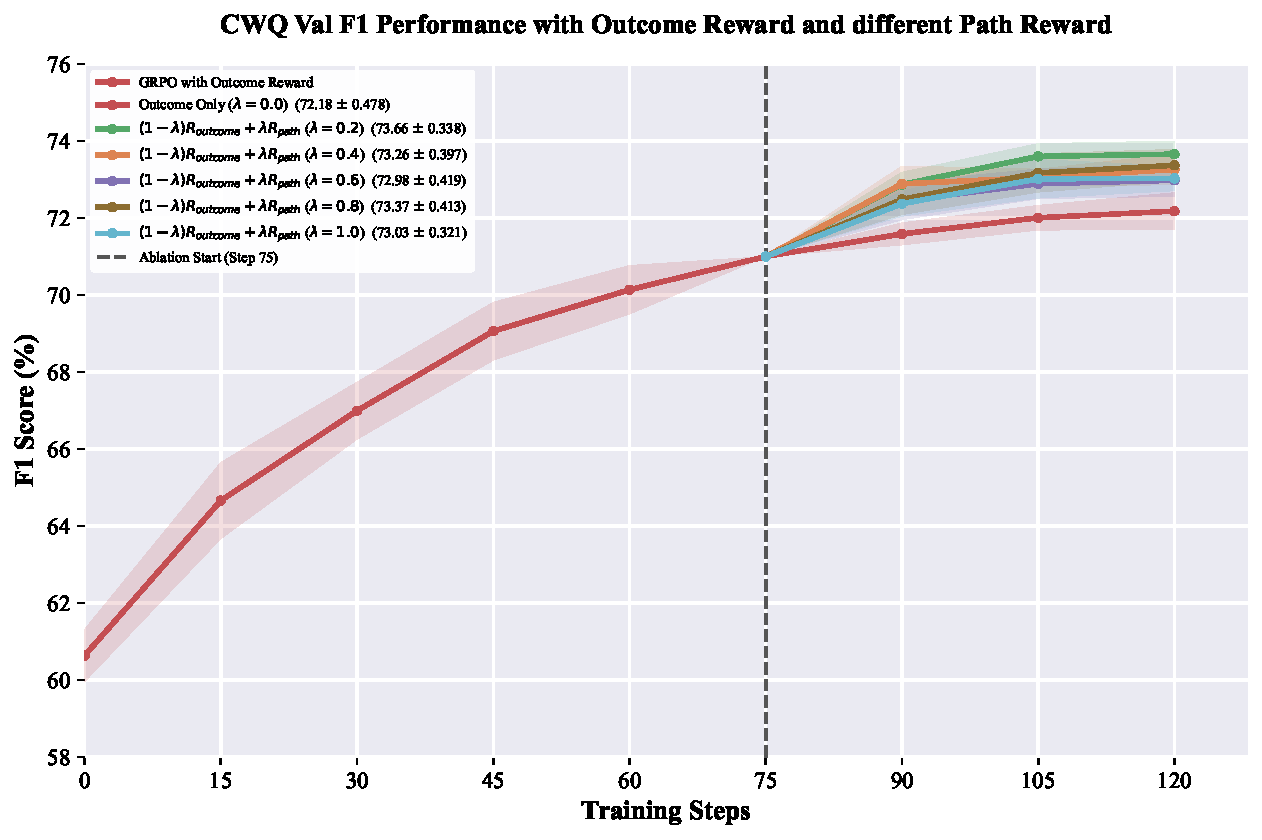
\includegraphics[width=0.9\linewidth]{figures/appendix/f1_path_ratio_spaced.pdf}
    \caption{Validation F1 performance on the CWQ dataset with varying Path Reward weights. The total reward is formulated as $R =(1-\lambda)R_{outcome} + \lambda R_{path}$, where $\lambda$ denotes the coefficient shown in the legend. The dashed vertical line marks the start of the second training phase at step 75, where the reward shifts from result-only RL to a mixed result-and-path reward. Solid lines and shaded regions represent the mean and standard deviation across 3 random seeds, respectively. The results indicate that $\lambda=0.2$ achieves the optimal balance, yielding the highest F1 score and robust stability compared to the baseline ($\lambda=0.0$).}
    \label{fig:seed-pdf}
\end{figure}


\section{Construction of Ground-Truth Reasoning Paths}
For datasets lacking explicit reasoning paths (e.g., WebQSP, CWQ, GrailQA, and QALD10-en), we constructed ground-truth paths ($r_{g}$) using a two-stage "Search-and-Verify" pipeline. This process bridges the gap in existing benchmarks by deriving reliable reasoning chains from raw Question-Answer (QA) pairs.
\textbf{Path Retrieval via Breadth-First Search (BFS).}
We first employed BFS on the Knowledge Graph to retrieve all potential topological paths connecting the topic entity (identified in the question) to the ground-truth answer entity. This step ensures high recall of potential reasoning chains.
\textbf{Semantic Verification via LLM.}
Since BFS often yields "spurious paths"—paths that are topologically valid but logically unrelated to the question—we utilized an LLM (Gemini-2.5-Flash) as a semantic filter. The LLM was prompted to evaluate whether each retrieved path logically corresponds to the semantic intent of the natural language question. Only paths that passed this semantic verification were retained as $r_{g}$ for calculating $R_{path}$.

Consequently, this approach provides the necessary supervision signals for the second-stage RL training, addressing the lack of $r_g$ in open-source benchmarks.

\section{Detailed Definition of Exploration Metrics}
\label{appendix:exploration_metrics}

To provide a fine-grained analysis of exploration behavior, we parse the 
triples mentioned in the model's reasoning trace (the \texttt{<think>} block) 
on the CWQ test set.

Let $\mathcal{D}$ denote the test set with size $N = |\mathcal{D}|$. 
For the $i$-th question, let $T_{pred}^{(i)}$ be the set of valid unique 
triples extracted from the model's reasoning path, and 
$T_{gold}^{(i)}$ be the set of triples in the ground-truth reasoning path.

\textbf{Exploration Efficiency ($\downarrow$).}
This metric measures the search overhead, representing the average number of triples the model explores to identify one correct reasoning triple. 
A lower value indicates higher efficiency, implying less wasted exploration effort for each valid discovery.
It is calculated as the mean ratio of total extracted triples to the number of correct triples found:

\begin{equation}
    \textbf{Exploration Efficiency} = \frac{1}{N} \sum_{i=1}^{N} 
    \frac{|T_{pred}^{(i)}|}
    {|T_{pred}^{(i)} \cap T_{gold}^{(i)}|}
\end{equation}

\textbf{Coverage of the Reasoning Space ($\uparrow$).}
To define this metric, we first conceptualize the Reasoning Space for a given question as the set of all potential valid paths within the Knowledge Graph that connect the starting entity to the target answer entities. Consequently, this metric measures the reasoning recall, quantifying the average proportion of the ground-truth logical chain (a subset of the reasoning space) that is successfully uncovered by the model's exploration.
A higher value indicates better coverage, meaning the model finds more of the required logical steps.
It is calculated as:
\begin{equation}
    \textbf{Coverage} = \frac{1}{N} \sum_{i=1}^{N} 
    \frac{|T_{pred}^{(i)} \cap T_{gold}^{(i)}|}
    {|T_{gold}^{(i)}|}
\end{equation}
